\documentclass[10pt, openany]{book}

\usepackage[sc]{mathpazo}
\linespread{1.03}
\usepackage[a4paper,width=150mm,top=25mm,bottom=25mm]{geometry}
\usepackage{booktabs}
\usepackage{float}
\usepackage{array}
\usepackage[T1]{fontenc}
\usepackage[utf8]{inputenc}
\usepackage{microtype}
\usepackage[english]{babel}
\usepackage{hyperref}
\usepackage[usenames,dvipsnames,table,xcdraw]{xcolor}
\usepackage[hang,small,labelfont=bf,up,textfont=it,up]{caption}
\usepackage[normalem]{ulem}
\usepackage{setspace}
\usepackage{fancyhdr}
\usepackage{soul}
\usepackage{graphicx}
\usepackage{pdfpages}
\usepackage{parskip}
\usepackage{tikz}
\usepackage[toc]{glossaries}
\usepackage[toc,page]{appendix}
\usetikzlibrary{positioning,arrows}
\usepackage[space]{grffile}

\usepackage{minted}
\usemintedstyle{autumn}
\setminted{framesep=2mm, frame=lines}

\usepackage[style=authoryear,natbib=true,backend=biber]{biblatex}
\addbibresource{biblio.bib}
\setlength\bibitemsep{0.5\baselineskip}

\pagestyle{fancy}
\fancyhf{}
\fancyhead[L]{Design and Implementation of an Adv. Rendered Screensaver}
\fancyhead[R]{By James Balajan}
\fancyfoot[C]{\thepage}
\renewcommand{\headrulewidth}{1pt}
\renewcommand{\footrulewidth}{1pt}
\fancypagestyle{plain}{
\pagestyle{fancy}}

\graphicspath{ {images/} }

\urlstyle{rm}

\makeglossaries

\newglossaryentry{atmospheric-scattering}
{
	name={Atmospheric Scattering},
	text={atmospheric scattering},
	description={Atmospheric scattering, in the context of computer graphics, refers to the modeling and emulation of the process by which light particles are scattered by particles in the atmosphere. Scattering from these particles leads to the blue color of our sky at noon, and its orange color at dawn and dusk}
}

\newglossaryentry{pbr}
{
	name={Physically Based Rendering},
	text={physically based rendering},
	description={In its broadest sense, physically based rendering refers to the usage of physics equations to accurately emulate the trajectories of photons when in contact with materials. An example of a physically based lighting model is the Cook-Torrance model, as opposed to the old, non-physically based Blinn-Phong model}
}

\newglossaryentry{volumetric-clouds}
{
	name={Volumetric Clouds},
	text={volumetric clouds},
	description={Volumetric clouds are rendered using the technique of \gls{volumetric-raymarching} over real-time generated volumes that are designed to emulate the shapes and behaviours of clouds}
}

\newglossaryentry{volumetric-raymarching}
{
	name={Volumetric Raymarching},
	text={volumetric raymarching},
	description={Volumetric raymarching is a graphics technique used to accurately render \gls{participating-media}, such as smoke, fog and clouds}
}

\newglossaryentry{participating-media}
{
	name={Participating Media},
	text={participating media},
	description={Participating media are materials which may absorb, emit and/or scatter light. Participating media usually consist of many particles suspended in the air}
}

\newglossaryentry{shader}
{
	name={Shader},
	text={shader},
	description={a type of computer program originally run on graphics card to do shading, aka lighting simulation. However, shaders now perform a variety of tasks, and the term now refers to a category of computer programs that are designed to be interpreted and run by the graphics card}
}

\newglossaryentry{OpenGL}
{
	name={OpenGL},
	description={a cross-language, cross-platform API standard for rendering 2D and 3D vector graphics. The API is used to interact with a graphics processing unit, to achieve hardware-accelerated rendering}
}

\newglossaryentry{GLSL}
{
	name={GLSL},
	description={GLSL (GLslang) is a short term for the official OpenGL Shading Language. GLSL is a C/C++ similar high level programming language for several parts of the graphic card. With GLSL you can code (right up to) short programs, called shaders, which are executed on the GPU}
}

\newglossaryentry{Assimp}
{
	name={Assimp},
	description={Open Asset Import Library is a cross-platform 3D model import library which aims to provide a common application programming interface for different 3D asset file formats.}
}

\newglossaryentry{component} {
	name={Component (Design Pattern)},
	description={Allow a single entity to span multiple domains without coupling the domains to each other. \citep{nystrom2014game}}
}

\newglossaryentry{Flyweight} {
	name={Flyweight (Design Pattern)},
	description={A flyweight is an object that minimizes memory usage by sharing as much data as possible with other similar objects; it is a way to use objects in large numbers when a simple repeated representation would use an unacceptable amount of memory. \citep{gamma1995design}}
}

\newglossaryentry{coupling} {
	name={Coupling},
	description={In software engineering, coupling is the degree of interdependence between software modules; a measure of how closely connected two routines or modules are. Low coupling is often a sign of a well-structured computer system and a good design, and when combined with high cohesion, supports the general goals of high readability and maintainability.}
}

\begin{document}

\pagenumbering{gobble}
\thispagestyle{empty}
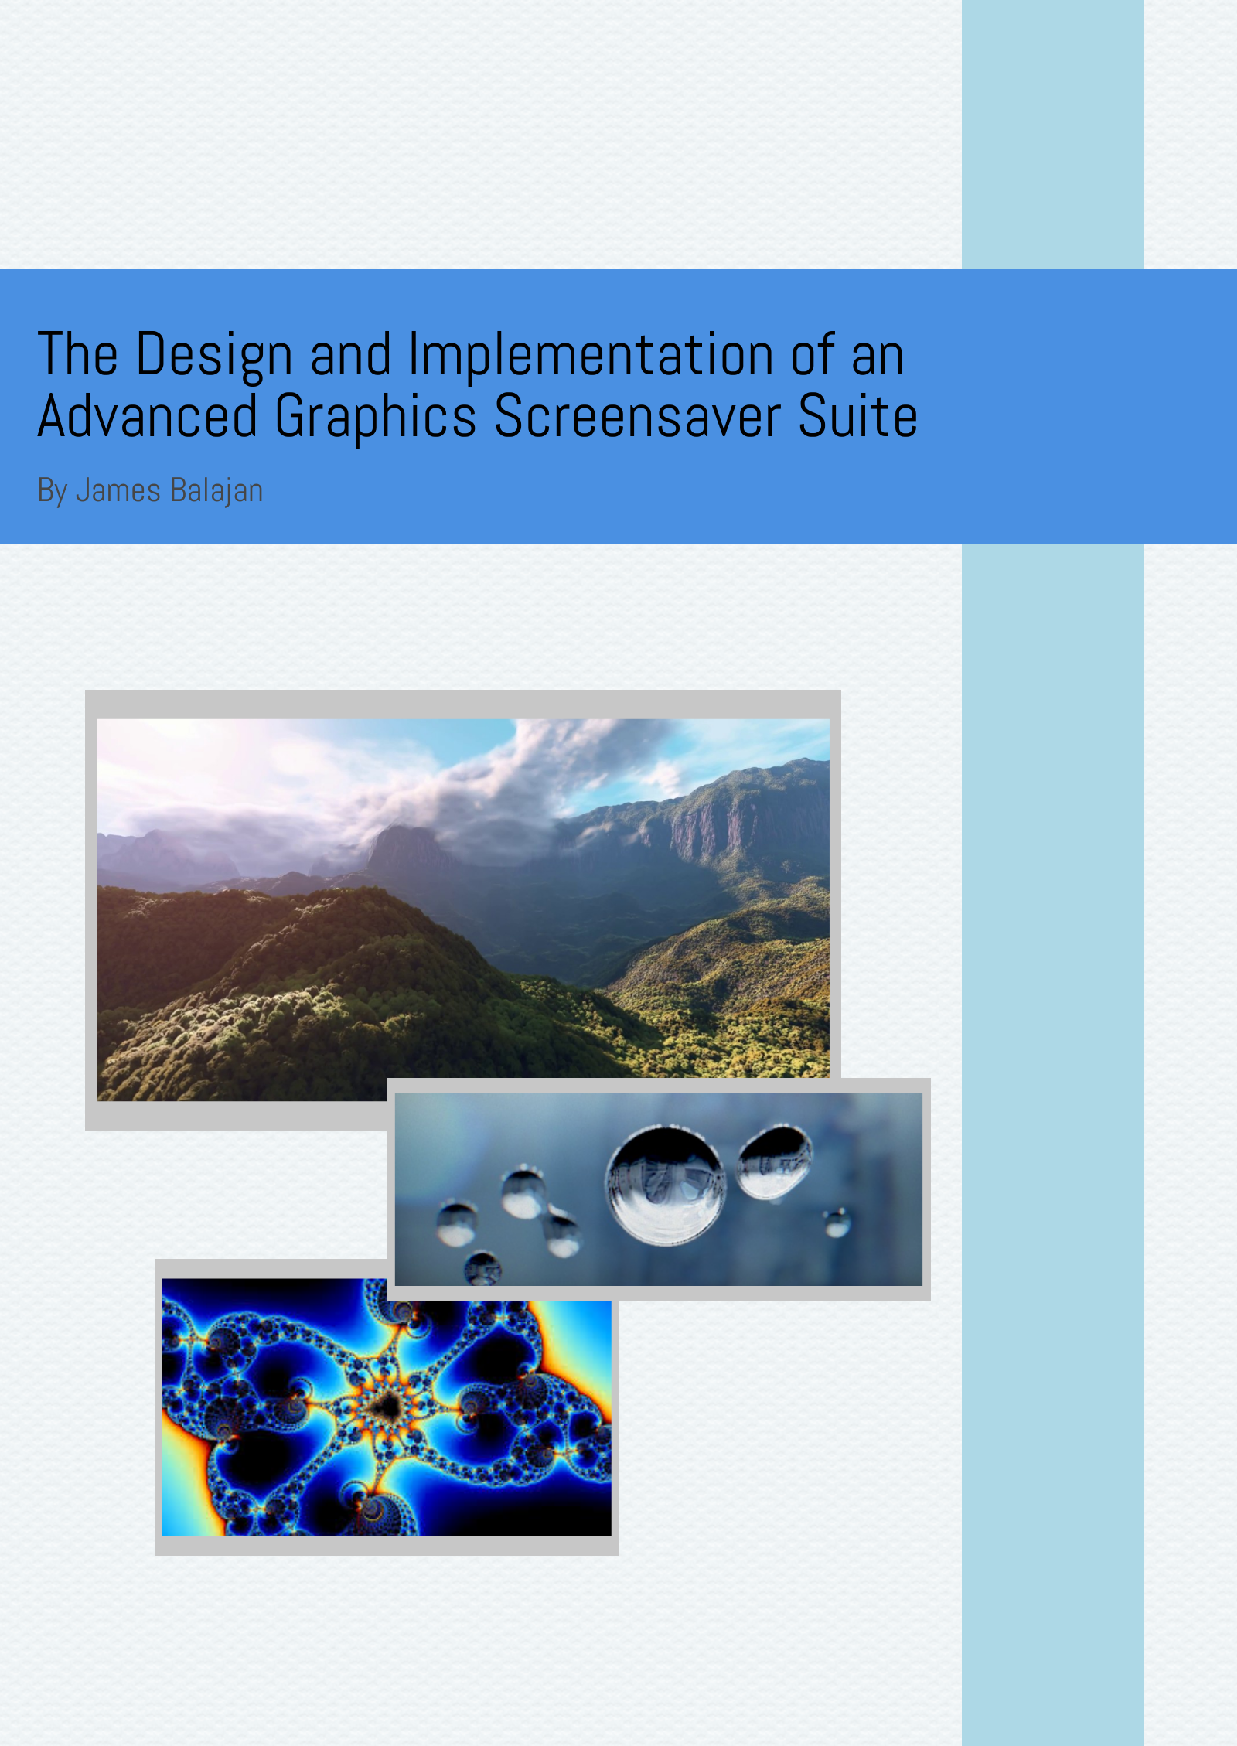
\includepdf{external-pdfs/titlepage.pdf}
\pagenumbering{roman}

\tableofcontents
\newpage

\listoffigures
\newpage

\pagenumbering{arabic}

\chapter{Project Proposal}

\begin{figure}[H]
        \centering
        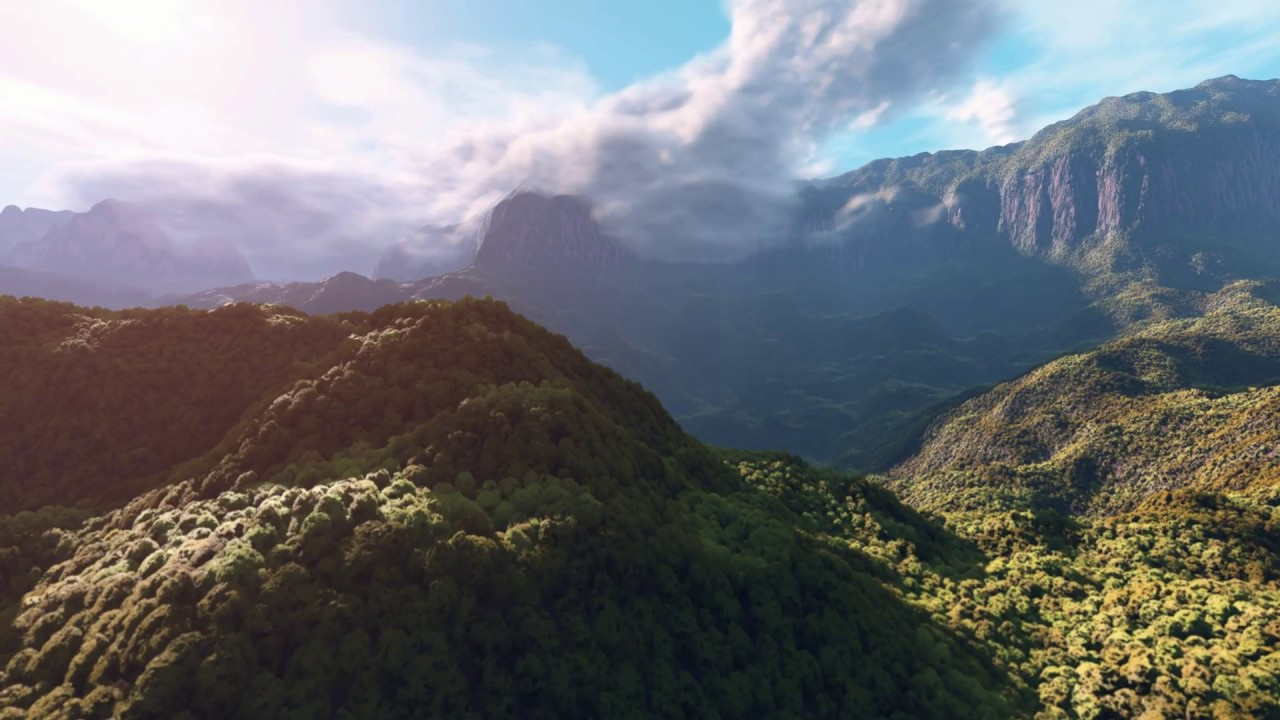
\includegraphics[width=0.35\linewidth]{rainforest}
        \caption{Inspiration for Screensaver. Computer generated Rainforest by Inigo Quilez}
\end{figure} 

\section{Executive Summary}
Much promise has been shown in the applicability of basic, computer generated graphics for creating screen savers for computers in the past, an example of this being that all of the screensavers for Windows XP were rendered. The ability to create aesthetically pleasing, dynamic graphics has made computer generated graphics find use in this field. For this reason a study will be undertaken to investigate if utilising advanced computer graphics techniques to generate a visually appealing scene, which will act as a screensaver, is possible without being overly burdensome on the computer's hardware. Some proposed techniques to be utilised to make this scene are \gls{pbr}, \gls{atmospheric-scattering} and \gls{volumetric-raymarching}, though this list of techniques is subject to change throughout the project as the needs and challenges of the project cannot fully be anticipated.

\begin{figure}[H]
        \begin{tikzpicture}
            [%%%%%%%%%%%%%%%%%%%%%%%%%%%%%%
                node distance=1cm,
                box1/.style={rectangle,draw,fill=white!10, very thick,
                              minimum width=3cm, minimum height=1cm},
                box2/.style={align=left,rectangle,draw,fill=gray!10, very thick,
                              minimum width=3cm, minimum height=4cm},
                line/.style={-latex,very thick}
            ]%%%%%%%%%%%%%%%%%%%%%%%%%%%%%%

        \node[box1]             (A) {Screensaver};
	\node[box1, below=of A] (B) {\Gls{pbr}};
	\node[box1, left=of B ] (C) {\Gls{atmospheric-scattering}};
	\node[box1, right=of B] (D) {\Gls{volumetric-clouds}};

        \draw[line] (A.west)  -| (C.north);
        \draw[line] (A.south) -| (B.north);
        \draw[line] (A.east)  -| (D.north);

        \end{tikzpicture}
\caption{Graphics techniques that may be used}
\end{figure} 

To manage the project, the structured approach will be utilised and documented in a portfolio. Our clientele would like for us to use VB.NET to create the project, so the project will be programmed utilising it. As a result, challenges may be faced regarding the performance of the screensaver. Since the development of this screensaver will be only undertaken by one developer, the anticipated completion date of the project is June 2019, although this deadline is subject to change based on circumstances regarding the project.

\chapter{Project Plan}
\section{Defining and Understanding the Problem}
Our initial thoughts on what software construction methodology to use leaned towards one which would benefit a small development team, such as the prototyping methodology. However, it is mandated by our project sponsor that a portfolio be developed to document our development process in a structured manner, so a structured approach is the best choice due to its reliance on documentation.

Thus, the project will be split into 5 stages according to the structured approach:
\begin{itemize}
	\item Planning
	\item Design
	\item Building / Implementing
	\item Testing
	\item Deployment	
\end{itemize}	

These stages are reflected in our Gantt Chart.
Please see figure \ref{fig:gantt} on page \pageref{fig:gantt} for the Gantt Chart.

During the design phase, a survey will be conducted, asking customers what features they would like in a screensaver suite. The survey responses will be considered in our designs and implementation.
After initial implementation, a survey will be conducted requesting the opinions of our customers on the product. As of such, there will be some elements of the prototyping methodology in our approach as well, iterating over our initial product to improve it and satisfy the expectations of our customers. However, as stated previously, the methodology of development will be primarily structured.

\section{Design}
When developing the designs for the product, the following will be created.
\begin{itemize}
	\item A Context Diagram
	\item A Data Flow Diagram	
	\item A Structure Diagram
	\item High level flowcharts for key functions in the program.
	\item A Data Dictionary.
\end{itemize}	
All besides the data dictionary will be created before the implementation stage. The data dictionary will be created along with the product itself.  

\section{Implementation}
The implementation stage will firstly begin with a technical research stage. Advanced graphics techniques involve use of heavy amounts of mathematics, and as of such, research papers must be studied and cited.

After the initial research, implementation will commence. Testing will be done regularly as the project progresses, to ensure each module is functioning before moving onto the next one and to avoid the accumulation of errors. 

\section{Testing}
On completing the implementation, the screensaver suite will be tested on a variety of hardwares, to ensure it functions correctly on other GPUs. This is critical, as graphics \gls{shader}s may perform differently and possibly unexpectedly based on each graphics card provider's \gls{OpenGL} implementation.

\begin{figure}[H]
	\centering
	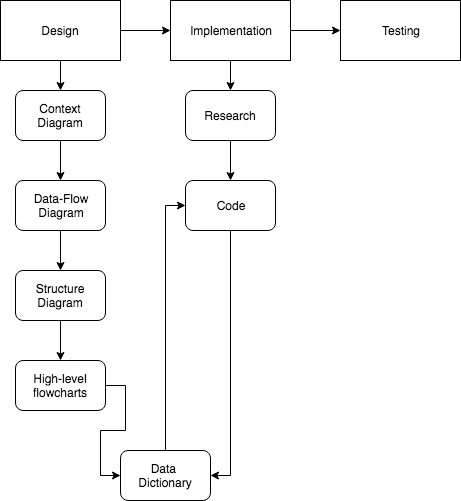
\includegraphics[width=0.6\linewidth]{project-plan}
	\caption{High-level diagram summarising project plan}
\end{figure}	

\chapter{Feasibility Study}

\section{Executive Summary}

Screensavers have been a medium of graphics experimentation during the times of early computing. However, advanced graphics techniques have never been applied to the context of screensavers, leaving an excellent vacant marketplace to test cutting edge techniques in the context of screensavers. This document analyzes the feasibility of undertaking a project where advanced graphics techniques are applied to create a screensaver from the lenses of technological feasibility, staffing feasibility and marketplace feasibility.

\section{Description of Products and Services}

Screensavers, during the times of early computing, have been the medium for the showcasing of various graphics techniques. From the Windows 98 era with the notable screensaver maze, bringing rasteurized graphics to the customer in a display of engineering creativity to the classic Windows XP pipes, using random generation to provide the customer with a new and consistently unique scene, graphics techniques have found their place in the world of screensavers. However, these screensavers have often been quite basic, using simple Phong shading or even no shading at all with only rasteur based techniques lacking lighting shading. This makes one wonder why advanced graphics techniques, such as the ones explored by video game companies and animation studies such as Pixar, have not been explored in the avenue of screensaver creation. 

\begin{figure}[H]
\centering
\begin{minipage}{.5\textwidth}
  \centering
  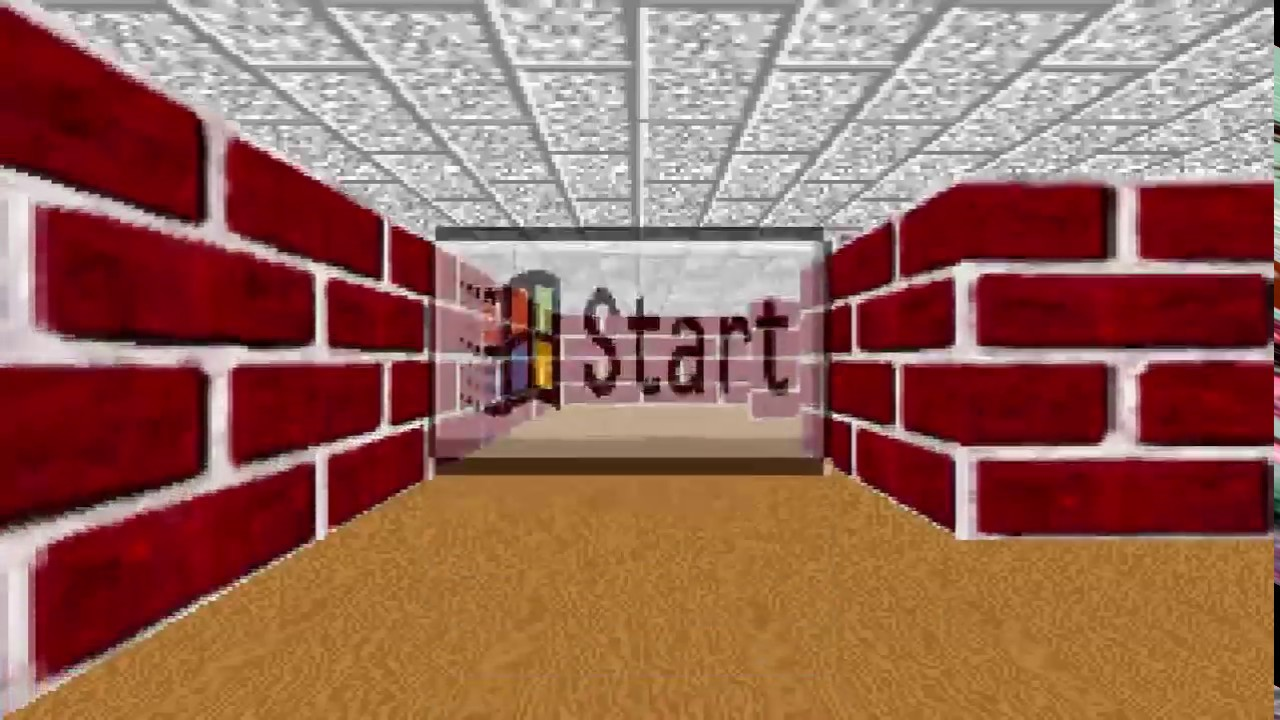
\includegraphics[width=.8\linewidth]{maze}
  \captionof{figure}{Windows 98 Maze}
\end{minipage}%
\begin{minipage}{.5\textwidth}
  \centering
  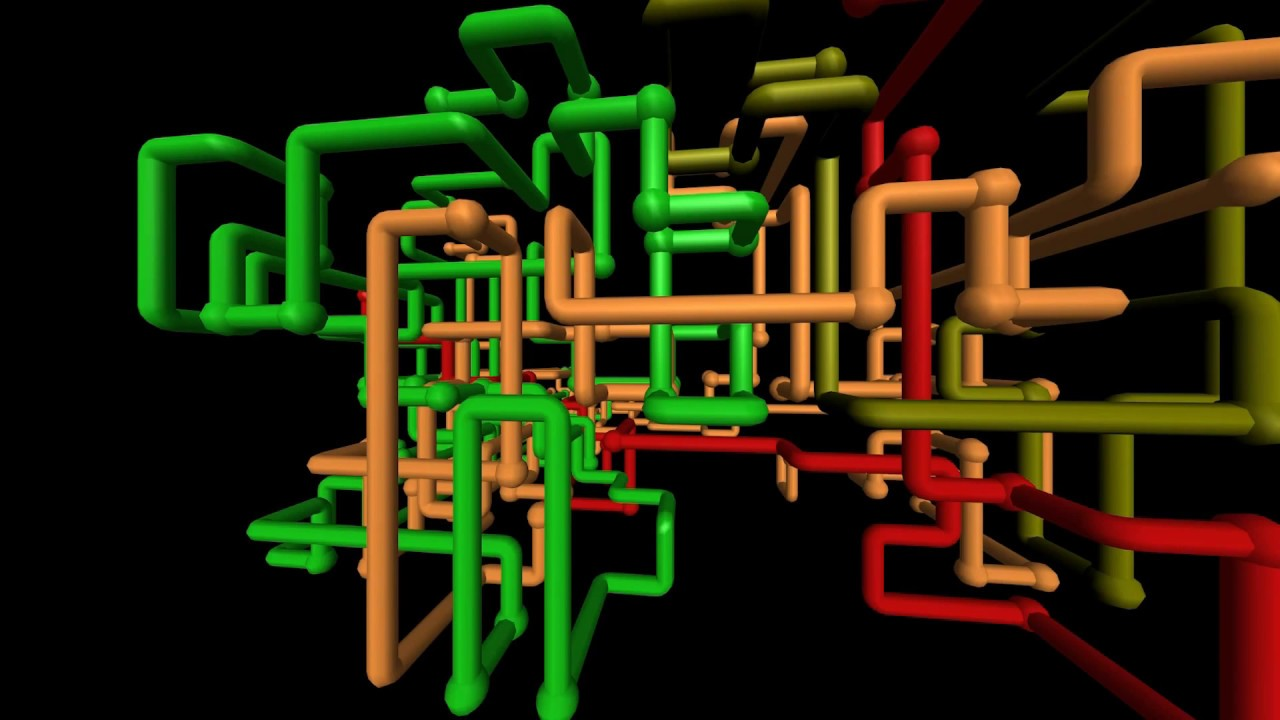
\includegraphics[width=.8\linewidth]{pipes}
  \captionof{figure}{Windows XP Pipes}
\end{minipage}
\end{figure}	

This project aims to investigate this avenue, with the aim of creating a suite of 3 screensavers. The first one will investigate the application of volumetric clouds and randomly generated terrain to screensavers. The second will investigate how mathematical fractal geometry may be applied to generating interesting screensavers. The final will investigate the application of the interesting effect of metaballs to screensavers. 

\begin{figure}[H]
\centering
\begin{minipage}{.3\textwidth}
  \centering
  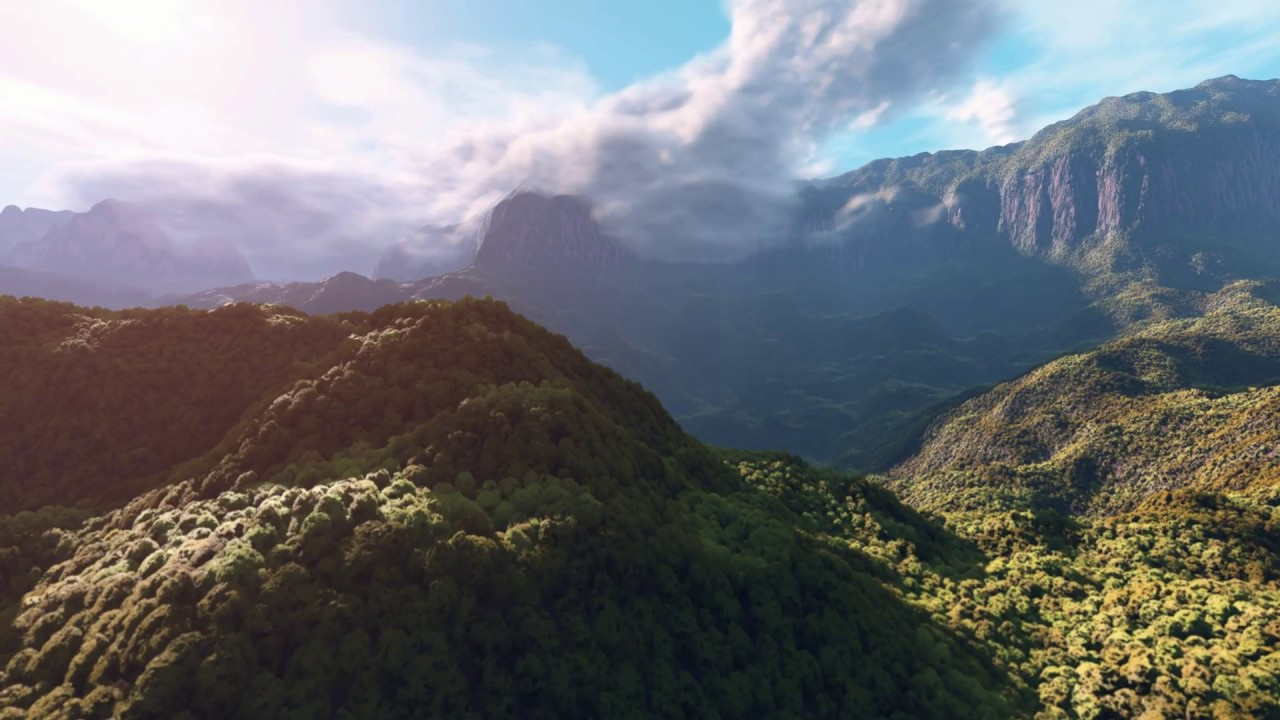
\includegraphics[width=.9\linewidth]{rainforest}
\end{minipage}%
\begin{minipage}{.3\textwidth}
  \centering
  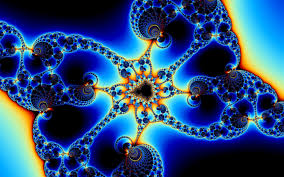
\includegraphics[width=.9\linewidth]{mandelbrot}
\end{minipage}%
\begin{minipage}{.3\textwidth}
  \centering
  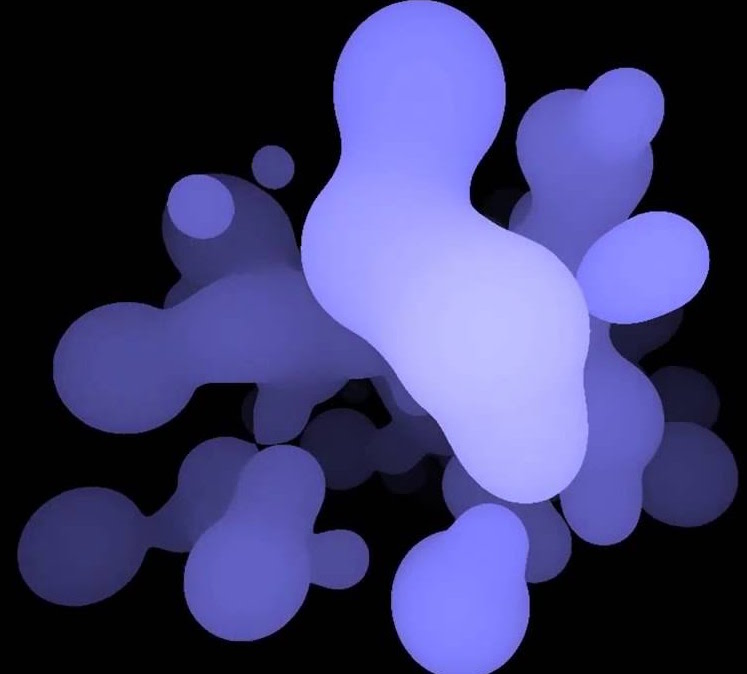
\includegraphics[width=.9\linewidth]{metaballs}
\end{minipage}
\caption{From left to right example images of: Terrain with Volumetric Clouds, Mandelbrot Fractal and Metaballs.}
\end{figure}	

\section{Technology Considerations}

\subsection{Hardware Considerations}

The personnel possess a single HP Pavilion laptop running Windows 10 OS that uses a Nvidia Geforce GTX 1050 graphics card. Although the graphics card is powerful, it is not out of reach of most customers, making it an excellent benchmark for what our users may use.

\subsection{Software Considerations}

The development will be carried out using the VB.NET programming language through the Visual Studio IDE. VB.NET was chosen as a matter of preference from our project sponsor. Due to this unorthodox choice for a programming language for graphics programming, in which C and C++ are most commonly used due to their performance, extra considerations may need to be taken regarding the overhead of the VB.NET language. Furthermore, as VB.NET is being used to create the screensaver suite, the project is only going to work on the Windows operating system as it required the .NET framework. However, projects such as .NET core and Mono aim to port the .NET framework to linux and mac, so cross compatibility is not completely out of the question, and can be implemented later if the demand is ever shown. 

\section{Product/Service Marketplace}

The marketplace for the utilisation of advanced graphics techniques in the context of screensavers has been fairly limited. No repositories on github were found for screensavers which utilised volumetric clouds, which is not surprising as it is a relatively new graphics technique which is still being researched. No procedural terrain screensavers were found either. This makes the first screensaver idea, of procedurally generated terrain with volumetric clouds, a venture into entirely uncharted territory, as the marketplace is entirely empty.

As for the mandelbrot fractal screensaver, mandelbrot fractals are well documented mathematical structures which produce beautiful results when rendered, however have also, surprisingly not been applied in the context of screensavers. There have, however, been large numbers of mandelbrot fractal explorers generated, as it is seen as an excellent exercise to develop one’s programming skills. An example written in Javascript is shown below:

\begin{figure}[H]
	\centering
	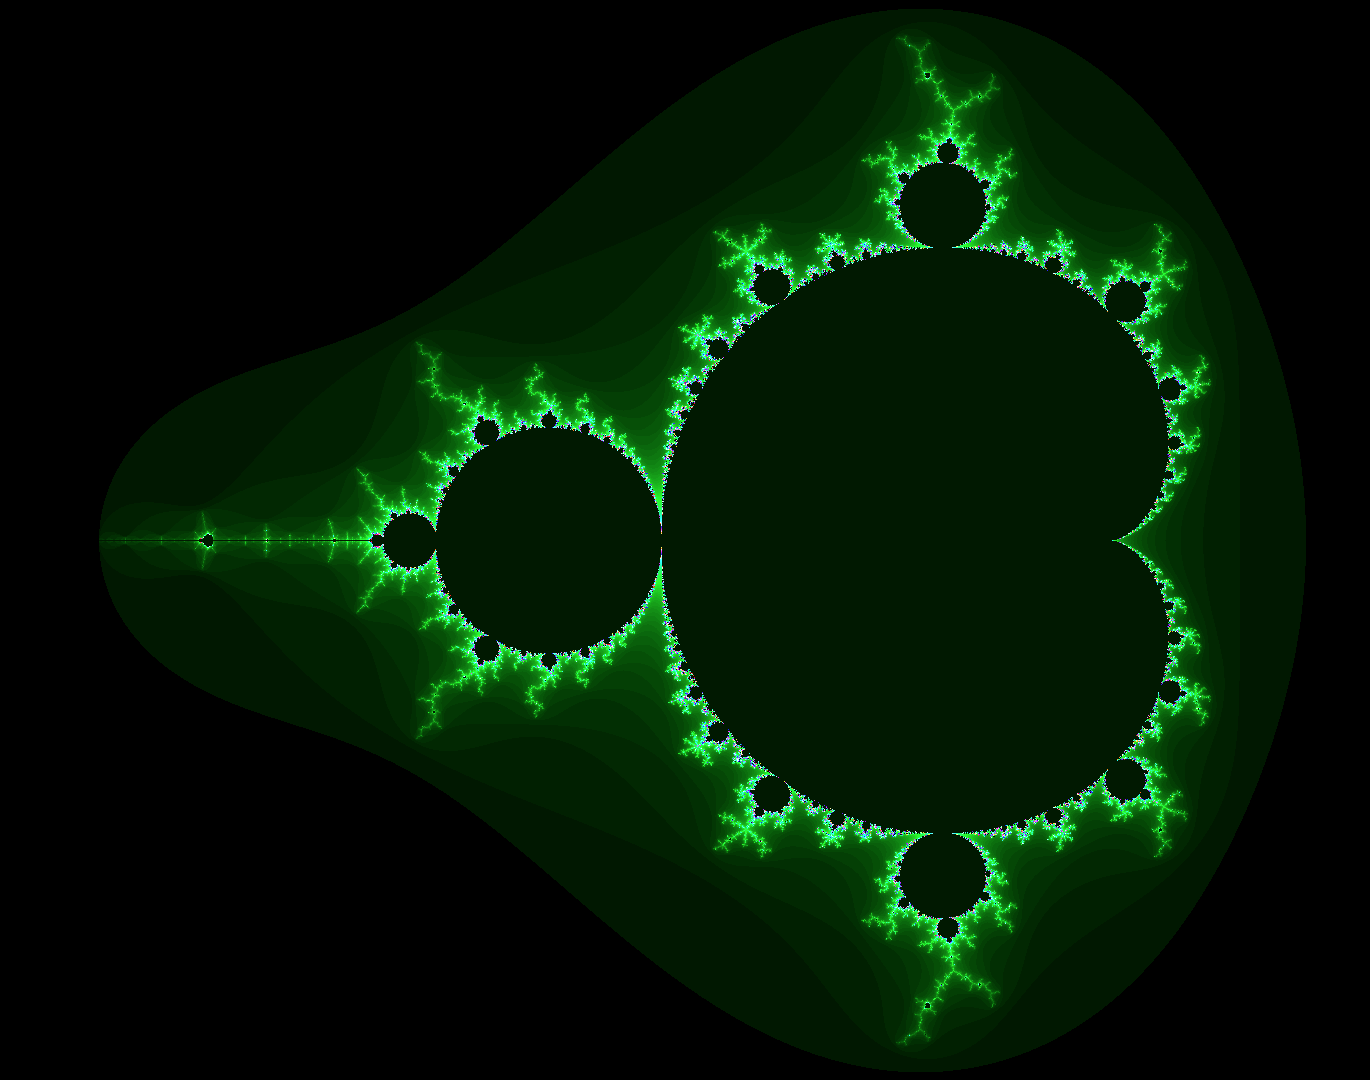
\includegraphics[width=.3\linewidth]{rafrex}
	\caption[Mandelbrot Fractal Rendered by Rafrex's "Fractal"]{Mandelbrot Fractal Renderered by Rafrex's "Fractal" from \url{https://github.com/rafrex/fractal}}
\end{figure}	

Metaballs are also a well documented technique, created by Jim Blinn, the father of Blinn-Phong shading, which produce organic looking balls that change shape depending on their positions relative to other metaballs. Metaballs have been applied to a wide range of areas, however, one particular use of them is in simulating the behaviour of water droplets efficiently, without the use of complex and expensive fluid dynamics simulations. Metaballs have not been applied to the context of screensavers, however, various eye candy demos have been created such as the one below written in Javascript:

\begin{figure}[H]
	\centering
	
\includegraphics[width=.3\linewidth]{dynaballs}
	\caption[Metaballs Rendered by FlannelHead's "Dynaballs"]{Metaballs Rendered by FlannelHead's "Dynaballs" from \url{http://flannelhead.github.io/dynaballs/}}
\end{figure}	

\section{Social and Ethical Considerations}

\subsection{Legal Considerations}
As this project is primarily a non-profit, research experiment, the project will be released using the Open Source MIT License. This license limits our liability and makes warranty not legally enforcable, legally protecting us in the case of a potential misuse of our software. The license permits commerical use, modification, distribution and private use of our not for profit, research project.

\subsection{Ergonomics}
\begin{itemize}
	\item The screensaver should be designed to be ergonomic and user friendly. This is easily achievable, as screensavers lack the traditional GUIs of many other products, their main purpose being to be eye candy. Options for these screensavers may be programmed to be directly accessible through the Windows control panel, or could be programmed to be configurable through a separate GUI all together.
	\item The design of the screensaver options dialog will aim to keep the interface simple and intuitive to use, not overflowing the user with unnecessary options. Advanced options will be hidden behind a drop down menu, for experienced users to utilise.
	\item The screensavers will aim to maximise FPS without jeopardising the quality of the screensavers.	
\end{itemize}	

\subsection{Inclusivity}
\begin{itemize}
	\item An English locale will be implemented into the screensaver
suite options dialog, as English is one of the most widely spoken languages in the world. Furthermore, a Russian locale will be implemented as it is the 7th most widely spoken language in the world, and the developer has knowledge of the language. As this project is open source, if more locales are desired to be programmed in, open source contributors may add them.
	\item Data formats that differ internationally, such as dates and currency, are not being handled and hence these factors do not need to be accounted for.
	\item The screensaver would be free and released under the open source licence, allowing anyone of any economic background to utilise it.
	\item The scenes rendered in the screensavers will be designed to be universally appealing to all demographics.	
	\item The option for the screensaver to play music may be programmed in at a later date. One option used to cater for people with hearing disabilities in software is to include subtitles. However, this solution is not suitable, as the person would still not be able to experience the music through a simple text prompt which says "Music Plays". As of such, this issue will be left open to the open source community to solve, if a solution is found in the future.
	\item People with visual impairments must also be catered for. Legal blindness cannot be catered for, as the product is a purely visual one. However, for people with mild visual impairments, text can be written using a clear serif or sans-serif font with a large font size. Poor color combinations will be avoided like yellow on white, only using colors which contrast well, such as black on white.
	\item Issues pertaining to cultural inclusivity need not be worried about, as the screensavers aim to have universal beauty, showcasing the remarkable natures of both the natural and mathematical worlds. 	
\end{itemize}	

\section{Organization and Staffing}

In considering to create this product, considerations must be made regarding whether the developers of this project possess the expertise and the technology required to complete the project. The development team consists of one student programmer, indicating that the personnel may lack the expertise required to develop an advanced graphics screensaver. However, the deadline for the end of the project provides enough time for the programmer to research and become knowledgable on these techniques before implementation.

\section{Schedule}

The schedule of this project will closely follow the Gantt Chart.
The structure of this gantt chart aims to reflect the standard software development life cycle.

\begin{figure}[H]
	\centering
	\makebox[\textwidth][c]{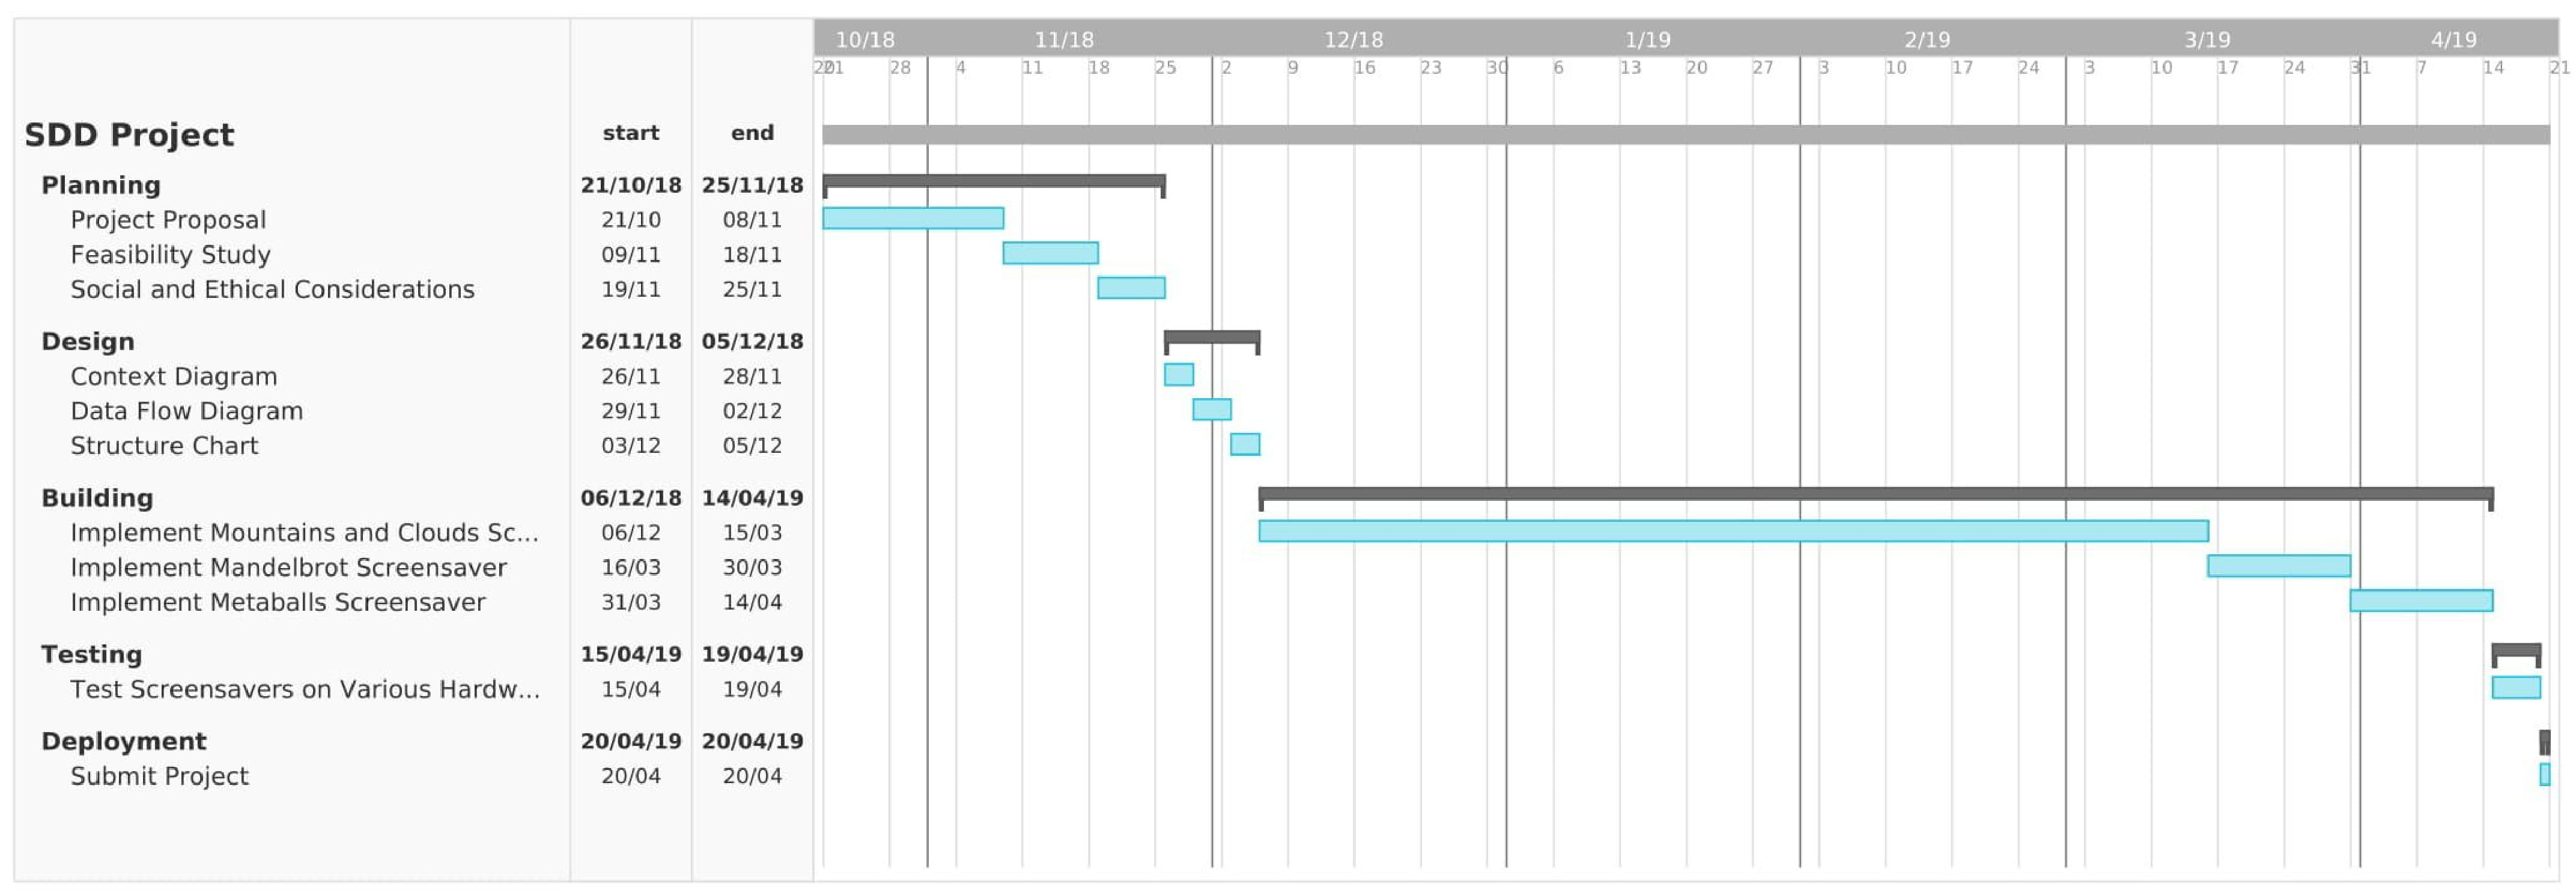
\includegraphics[width=1.2\linewidth]{gantt}}%
	\caption{Gantt chart}
	\label{fig:gantt}
\end{figure}	

\section{Financial Projections}

As the project manager is also the developer and has direct interests in completing this project, the developer demands no pay.
No extra software must be purchased, as all tools that will be used are free.
The only costs associated with this project are those associated with electricity for recharging the laptop.

\section{Findings and Recommendations}

In summary:
\begin{itemize}
	\item There is ample time for research, development and refinement.
	\item Through investigating advanced graphics techniques in screensavers, one can set the groundwork for their future integration into other mediums such as animated movies and video games.
	\item The cost of development is negligible.	
\end{itemize}	
Hence, it is in our best interests that the project proceed.

\chapter{Design}

\section{System Modeling Diagrams}
As a screensaver product is primarily visual, the first part of the design stage was to create an array of preliminary screen designs, with one for each of the three screensavers in the suite.
These screen designs may be found in the appendix according to the list below:
\begin{itemize}
	\item Clouds and Mountains Screen Design (pg. \pageref{app:clouds-screen})
	\item Mandelbrot Screen Design (pg. \pageref{app:mandelbrot-screen})
	\item Metaballs Screen Design (pg. \pageref{app:metaballs-screen})
\end{itemize}

In the design stage, a detailed context diagram, data flow diagram (DFD), structure chart and storyboard were also created for each of the three screensavers. Furthermore a data dictionary was created to catalogue the variables used in each of the three screensavers.

The data dictionary may be found on page \pageref{app:data-dictionary}.
The design diagrams may be found on their respective pages as shown in table \ref{tab:page-nums}.

\begin{table}[H]
\centering
\caption{Page Numbers of Design Documents}
\label{tab:page-nums}
\begin{tabular}{|l|l|l|l|l|}
\hline
Screensaver & \begin{tabular}[c]{@{}l@{}}Context Diagram \\ \\ Page No.\end{tabular} & \begin{tabular}[c]{@{}l@{}}DFD \\ \\ Page No.\end{tabular} & \begin{tabular}[c]{@{}l@{}}Structure Chart \\ \\ Page No.\end{tabular} & \begin{tabular}[c]{@{}l@{}}Story board Page \\ \\ No.\end{tabular} \\ \hline
Clouds and Mountains & \pageref{app:clouds-context} & \pageref{app:clouds-dfd} & \pageref{app:clouds-struc} & \pageref{app:clouds-story} \\ \hline
Mandelbrot & \pageref{app:mandelbrot-context} & \pageref{app:mandelbrot-dfd} & \pageref{app:mandelbrot-struc} & \pageref{app:mandelbrot-story} \\ \hline
Metaballs & \pageref{app:metaballs-context} & \pageref{app:metaballs-dfd} & \pageref{app:metaballs-struc} & \pageref{app:metaballs-story} \\ \hline
\end{tabular}
\end{table}

\section{Modularity and Design Patterns}
\subsection{Clouds and Mountains Screensaver}
When designing the clouds and mountains screensaver, careful attention was put into making an effective modular system, with each module only completing a certain task. By using these object-oriented design principles, each module is effectively able to be removed or added back to the screensaver easily, or even used for different purposes than initially intended as long as it is provided the required inputs, due to the layers of abstraction. Each module adheres to the \textit{\glslink{component}{Component}} design pattern as defined in \citep{nystrom2014game}, meaning that they are implemented classes which abstract the lower-level behaviour of higher level classes, to ensure modular design, clean code and to reduce the \glslink{coupling}{coupling} between different classes, meaning that the modules may be moved about and altered without causing the code to break. 

A detail not shown in the data flow diagram is the use of the \textit{\glslink{Flyweight}{Flyweight}} design pattern as defined in \citep{gamma1995design}, which was implemented to optimize RAM usage. The \textit{\glslink{Flyweight}{Flyweight}} design pattern allows for the screensaver to only need to store the model data once on RAM, whilst simultaneously allowing for customization of the trees so that the forest does not look repetitive. If each instance of a tree had its own model, the amount of data that would need to be stored on RAM would grow $O(n)$ with the number of trees drawn to the landscape. To put that in perspective, the tree model used in the screensaver uses 86886 vertices to draw the leaves alone. If a copy of this data were stored for every instance of a tree drawn, the screensaver would quickly run out of RAM. A pictorial representation of a forest without the \textit{\glslink{Flyweight}{Flyweight}} design pattern compared with a forest with the pattern is shown is show in figure \ref{fig:flyweight}. Notice how the optimized version does not contain duplicate data, with each tree instead referencing the same model, and altering it based on its parameters.

\begin{figure}[H]
\centering
\begin{minipage}{.46\textwidth}
  \centering
  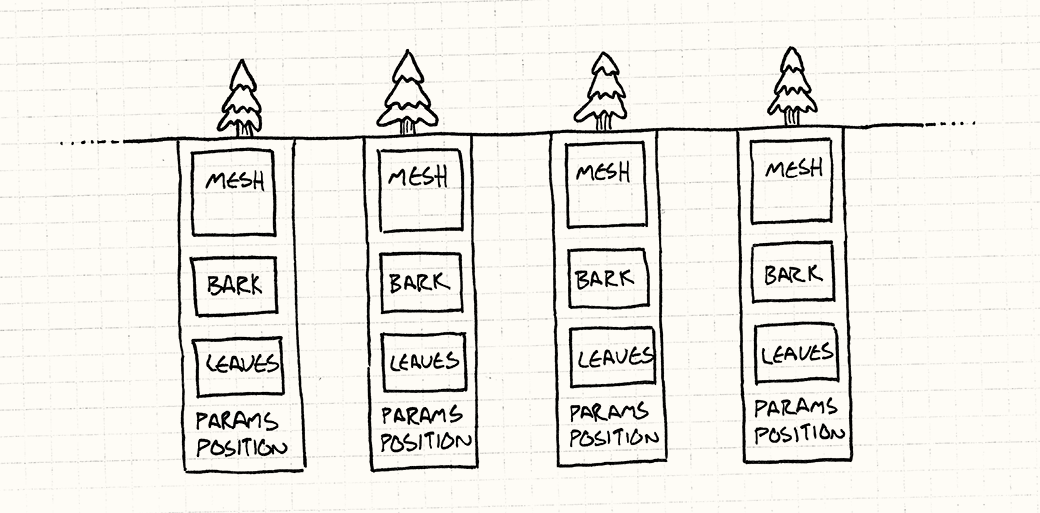
\includegraphics[width=.98\linewidth]{flyweight-trees}
\end{minipage}%
\begin{minipage}{.54\textwidth}
  \centering
  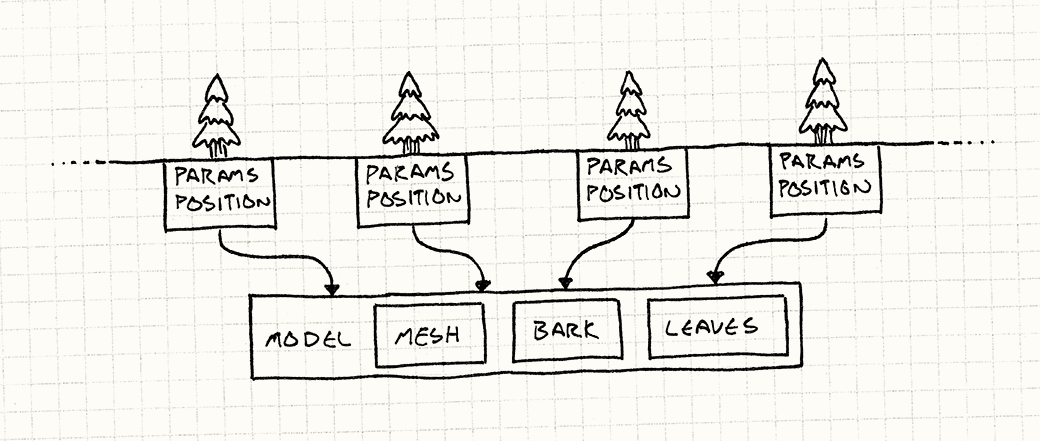
\includegraphics[width=.98\linewidth]{flyweight-tree-model}
\end{minipage}
\caption[Flyweight Forest]{A forest's storage without the \textit{\glslink{Flyweight}{Flyweight}} design pattern vs. with it. Sourced from \citep{nystrom2014game}}
\label{fig:flyweight}
\end{figure}	

This design pattern may be extended to even reducing the number of \Gls{OpenGL} draw calls, and vertex data being sent to and from the graphics card, using a feature in \Gls{OpenGL} called \textit{instancing}, which allows for only one draw call to be used to render all of the trees. Running \Gls{OpenGL} calls such as \mintinline{VB.NET}{GL.DrawElements} is more expensive than the actual drawing of the vertices, as \Gls{OpenGL} needs to always undertake the necessary preparations to make the data ready for consumption by the GPU, and must also transfer the data slowly along the bus from the CPU to the graphics card. \citep{learnOpenGLInstancing}. By compressing all of these draw calls into a single instance draw call, the data may be transferred to the graphics card in a single, contiguous packet, avoiding all of the overhead associated with multiple \Gls{OpenGL} calls. In this way, the design of the product was not only carefully created to ensure a clear and logical method of viewing the code with limited coupling, yet was also able to optimize the actual product itself.

\subsection{Mandelbrot Screensaver}
The mandelbrot screensaver's calculations occurred entirely on a \glslink{shader}{shader} program on the graphics card. However, some efforts were still made to ensure modularity within the program, for even simple programs can benefit from it. For instance, as seen in the data flow diagram (pg. \pageref{app:mandelbrot-dfd}), the configuration manager is placed in its own module which reduces the \glslink{coupling}{coupling} between the actual screensaver itself, and its settings.

Furthermore, a more subtle form of \glslink{coupling}{decoupling} occurs, in how the graphics code is separated from the management class in that it is stored in a shader. The two of them communicate using an \Gls{GLSL} feature called \textit{uniforms}, which are variables that are passed from the CPU to the graphics card via the bus every frame drawn. For instance, variables which are managed by the broader \textit{Screensaver} module, such as the system time, screen resolution, seed for the first zoom point and selected mandelbrot fractal palette are passed into the shader as defined by the uniforms:

\begin{minted}[framesep=2mm, frame=lines]{GLSL}
uniform vec3 iResolution;
uniform float iTime;
uniform int zoomPointSeed;
uniform int selectedPalette;
\end{minted}

\subsection{Metaballs Screensaver}
The metaballs screensaver is similarly designed to the mandelbrot screensaver, with the graphics calculations largely confined to its \glslink{shader}{shader} program. Like the mandelbrot screensaver, the metaballs screensaver too decouples its configuration manager from the main class. However it also decouples the physics calculations for each of the droplets into a droplet manager class as seen in the data flow diagram (pg. \pageref{app:metaballs-dfd}).

The metaballs screensaver shader is also decoupled from the main metaballs class, with it passing the center and radii of each droplet to the shader, as well as the height / amplitude of the waves, the system time and the screen resolution, as defined by the uniforms:

\begin{minted}[framesep=2mm, frame=lines]{GLSL}
uniform vec3 iResolution;
uniform float iTime;

uniform float waveHeight;

...

uniform vec3 dropletCenters[NUM_DROPLETS];
uniform float dropletRadii[NUM_DROPLETS];
\end{minted}

\section{User Feedback}
When creating the final designs for the screensaver suite, the project utilized user feedback based on iterative prototypes of the product that had been made. For instance, the decision to implement a configuration manager for the screensaver suite was derived from Arjun Malik's second survey response (pg. \pageref{app:survey-arjun-2}) as well as Julian Peen's second survey response (pg. \pageref{app:survey-julian-2}). This configuration manager manifests itself in the final data flow diagram for each of the three screensavers, as a "Config Manager" process.

The surveys also showed that personal preference still has an effect on screensaver choice, even when the screensavers are designed to be universally appealing. Samuel Stacy's second survey response (pg. \pageref{app:survey-sam-2}) showed that he did not dislike the mandelbrot fractal screensaver because of any technical or visual issue, yet simply due to personal preference. On asking him in person which screensaver he preferred the most, he said it was the clouds and mountains screensaver. This differed from other survey responses like, for instance, Ms Saki's (pg. \pageref{app:survey-aartee}), who stated that the metaballs screensaver was her favourite. This may have to do with people's subjective perceptions of beauty, for Samuel prefers the more realistic screensaver based on natural beauty, whilst some others prefer the abstract mathematical beauty of the mandelbrot fractal or metaballs. In this way, by creating a suite of three screensavers which contain both real and abstract beauty, the product is able to appeal to both of these preferences.

One suggestion which has been suggested to be added is the option for adding music to the screensaver, as shown in Ms Saki's survey response (pg. \pageref{app:survey-aartee}). This idea is very original, as screensavers have never, in the scope of the market survey conducted, included the option for playing music. However, there do exist some concerns regarding this feature's utility, as screensavers typically run when the user is not at their computer, meaning that there would be no one to receive the music, except for the user when they return from whatever activity removed them from the computer. Furthermore, concerns surrounding time are paramount as the project is beginning to reach its conclusion, as the screensavers must be tested on other architectures and fixed if any issues are present, meaning that there may not be enough time to both implement this new feature and complete the testing. If this feature is not added to the final product, and it is likely that it would not be, a future experiment should be conducted to observe both the market and technical feasibility of a screensaver which employs both visual and auditory stimuli. If this experiment goes well, auditory features may either be incorporated into the current product, or a new screensaver may be created which would better showcase the potential of an audio-visual screensaver.

All of the surveys conducted may be found in the appendix.

\section{Configuration Windows}

(TO DO: Screen designs)

The configuration windows were designed with usability and inclusivity in mind. All labels were given large font sizes to assist people with mild visual impairments with seeing the text. The sliders' values are displayed in the label as they change dynamically, allowing for the user to have a quantitative idea of how their settings have changed. On quitting the configuration window without saving, the application will open a message box, asking the user if they want to quit without saving their settings to prevent loss of settings. The appropriate question mark icon is used in this message box, as it is asking the user for input, rather than displaying an error message or a warning.

\begin{figure}[H]
	\centering
	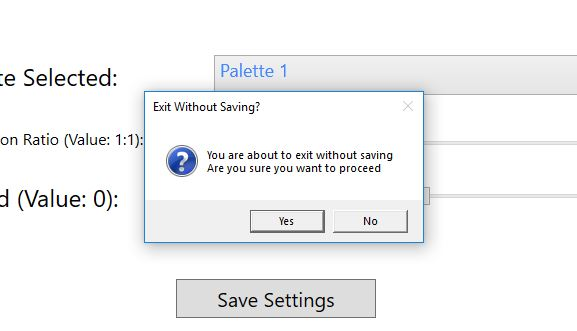
\includegraphics[width=.5\linewidth]{ExitWithoutSaving}
	\caption[Configuration Window Message Box]{Message Box Which Appears on Not Saving Configuration Settings}
\end{figure}	

(TO DO: TALK ABOUT LOCALE)


\printbibliography[heading=bibintoc,title={Bibliography}]

\printglossaries

\chapter{Appendix}
\section{Designs}
\subsection{Clouds Screensaver Context Diagram}
\begin{figure}[H]
	\centering
	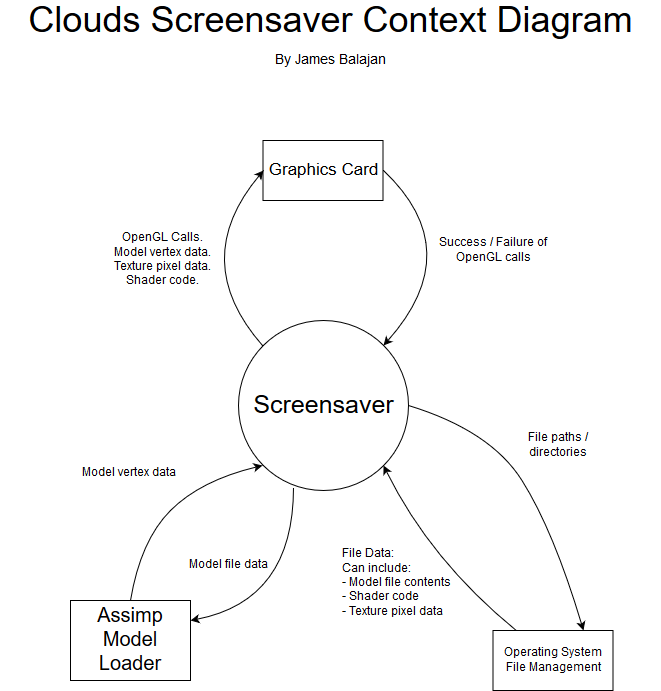
\includegraphics[width=0.9\linewidth]{Clouds Context Diagram}
	\caption{Clouds Screensaver Context Diagram}
	\glslink{Assimp}{}
	\label{app:clouds-context}
\end{figure}
\newpage

\subsection{Clouds Screensaver Data Flow Diagram}
\begin{figure}[H]
	\centering
	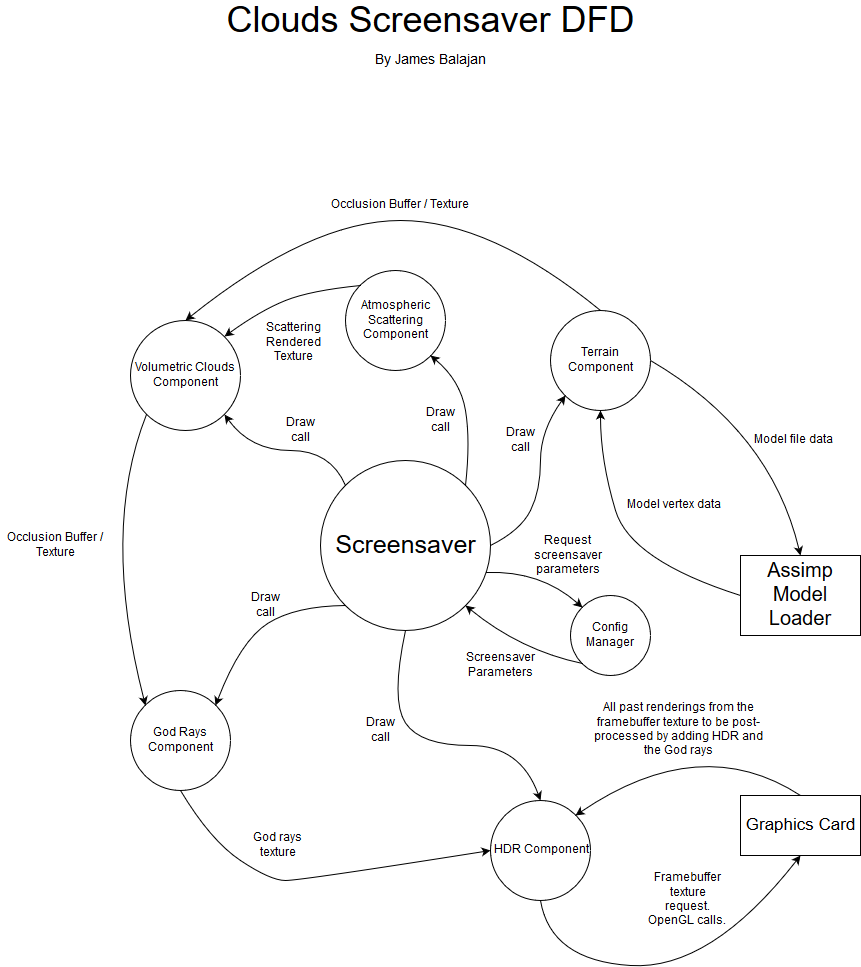
\includegraphics[width=1.0\linewidth]{Clouds Screensaver DFD}
	\caption{Clouds Screensaver Data Flow Diagram}
	\glslink{Assimp}{}
	\label{app:clouds-dfd}
\end{figure}
\newpage

\subsection{Clouds Screensaver Structure Chart}
\begin{figure}[H]
	\centering
	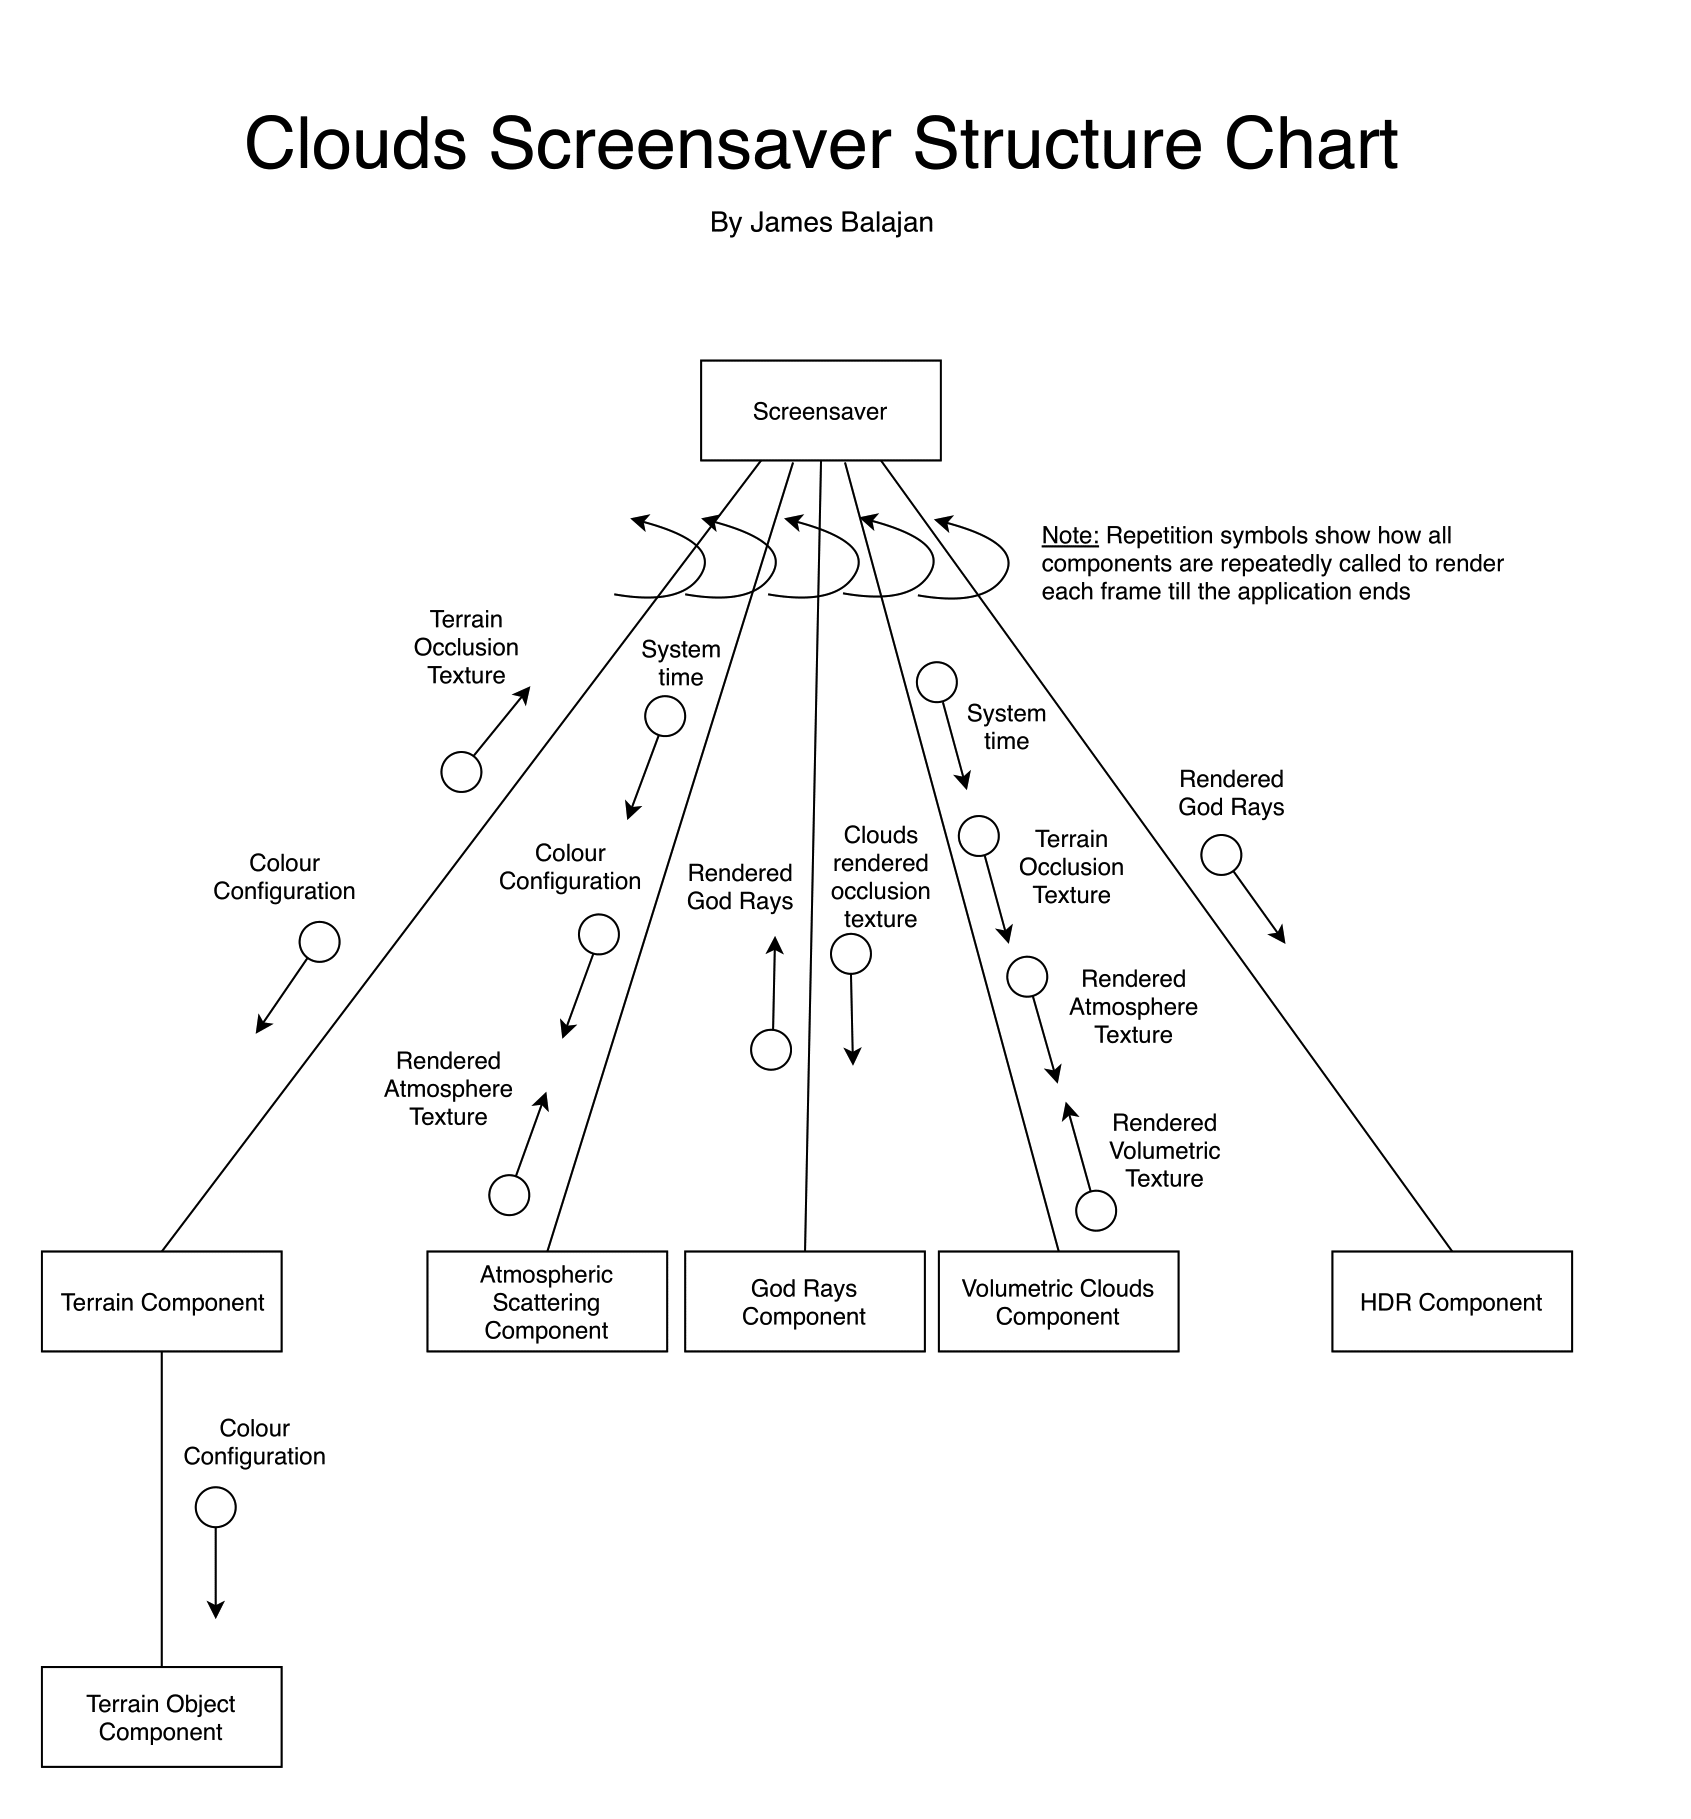
\includegraphics[width=1.0\linewidth]{Clouds Screensaver Structure Chart}
	\caption{Clouds Screensaver Structure Chart}
	\label{app:clouds-struc}
\end{figure}
\newpage

\subsection{Clouds Screensaver Storyboard}
\begin{figure}[H]
	\centering
	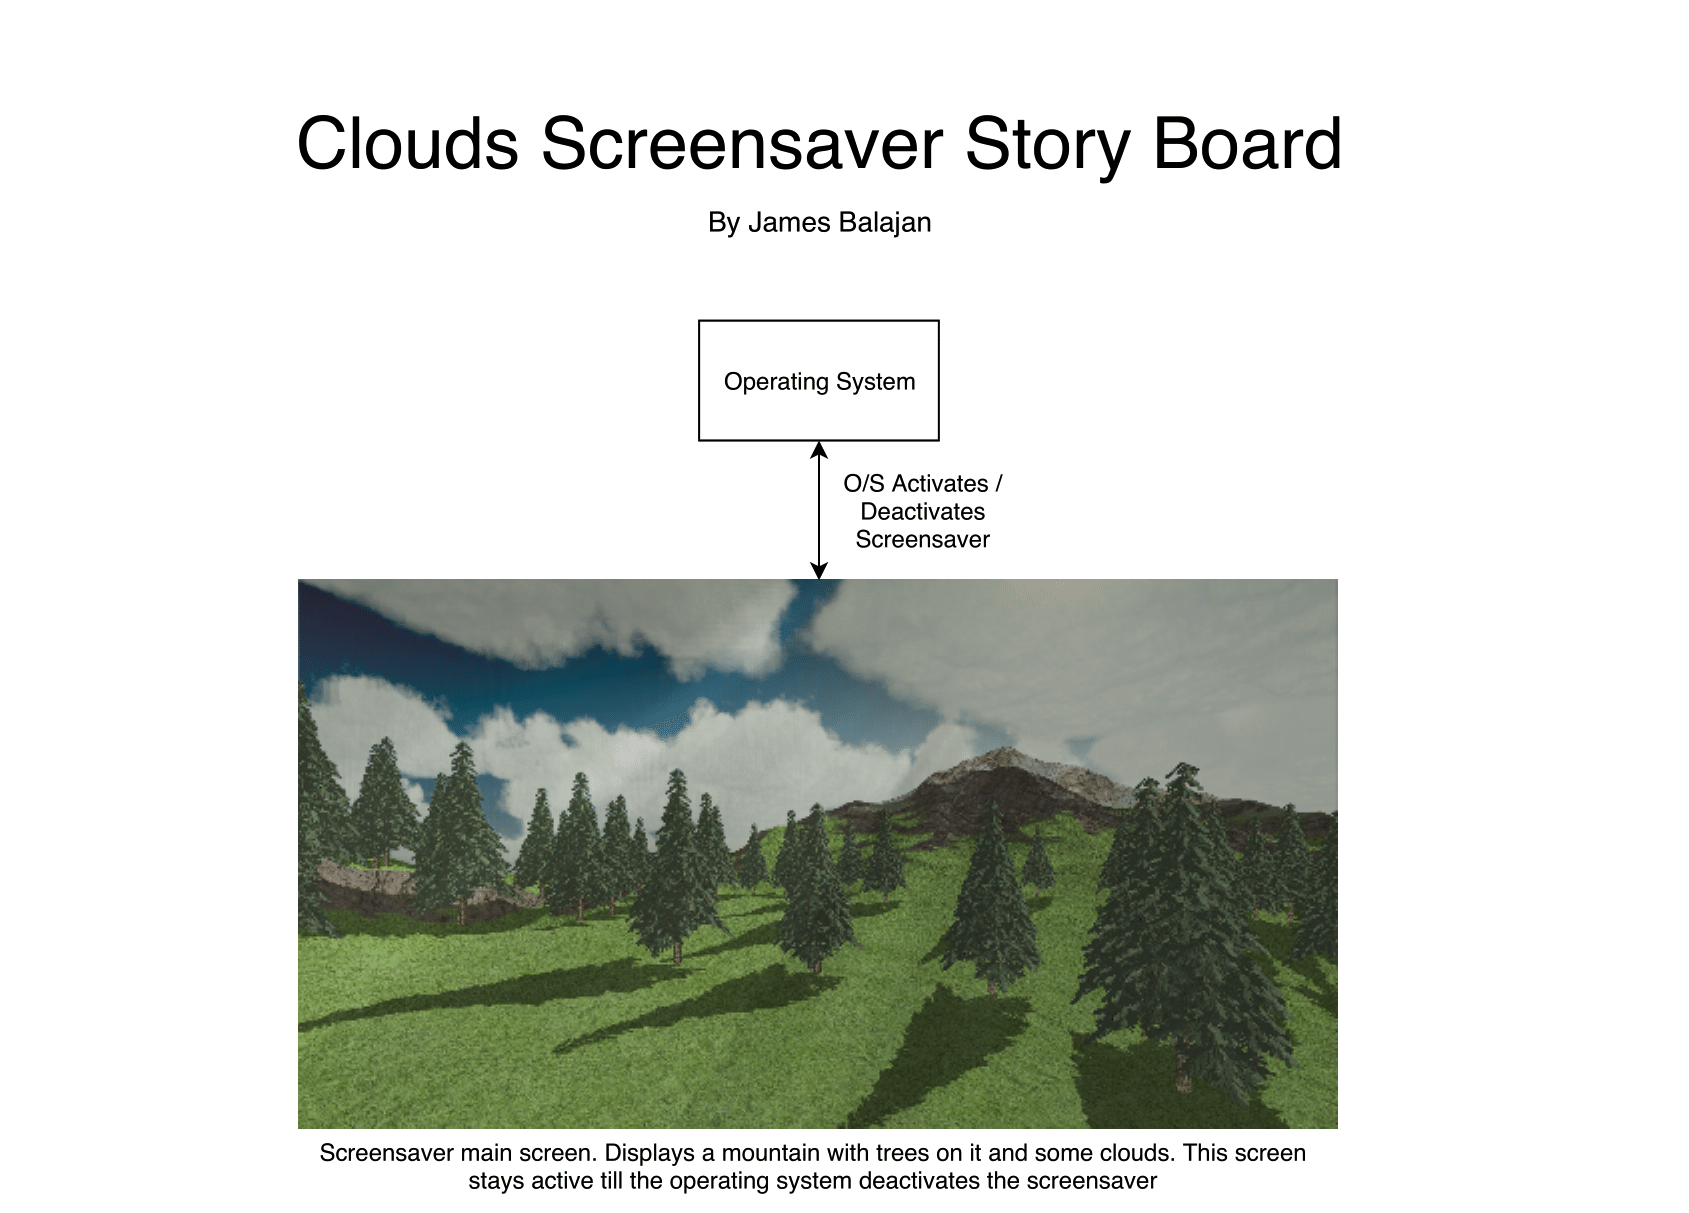
\includegraphics[width=1.0\linewidth]{Clouds Screensaver Storyboard}
	\caption{Clouds Screensaver Storyboard}
	\label{app:clouds-story}
\end{figure}
\newpage

\subsection{Mandelbrot Screensaver Context Diagram}
\begin{figure}[H]
	\centering
	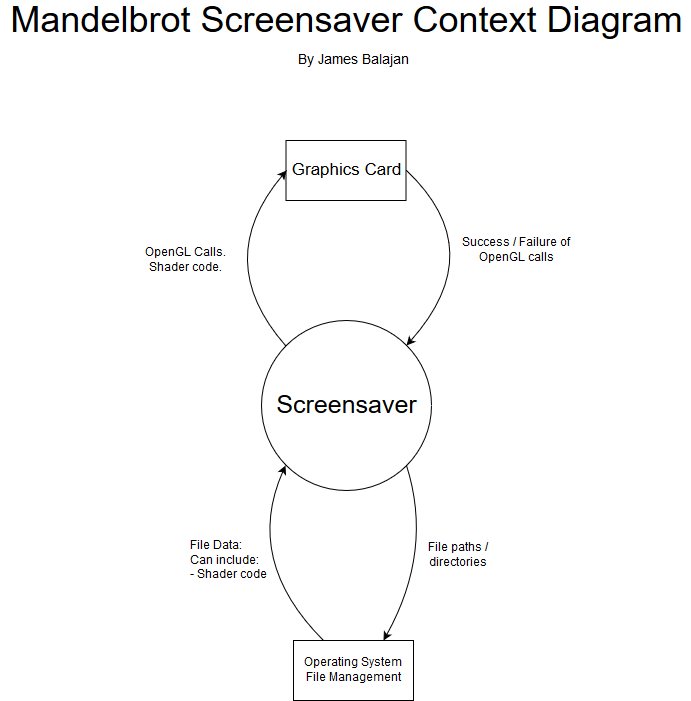
\includegraphics[width=1.0\linewidth]{Mandelbrot Screensaver Context Diagram}
	\caption{Mandelbrot Screensaver Context Diagram}
	\label{app:mandelbrot-context}
\end{figure}
\newpage

\subsection{Mandelbrot Screensaver Data Flow Diagram}
\begin{figure}[H]
	\centering
	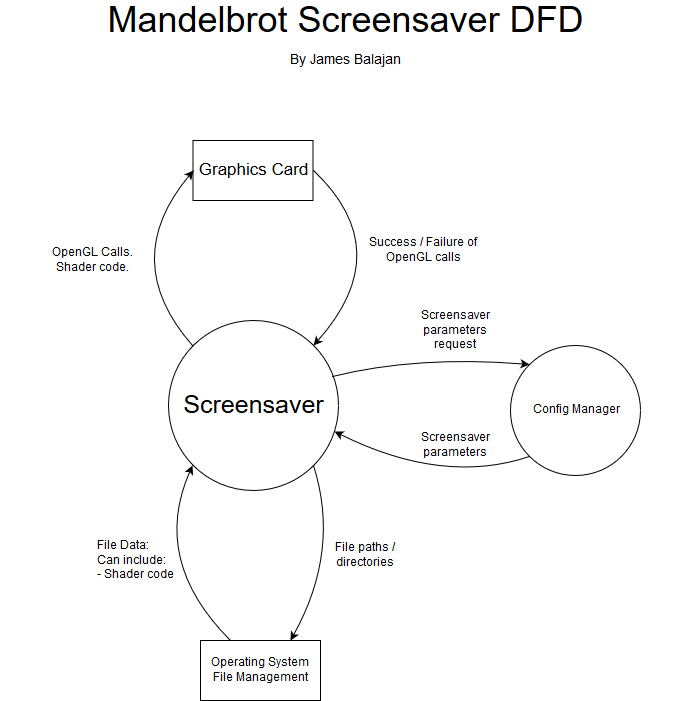
\includegraphics[width=1.0\linewidth]{Mandelbrot Screensaver DFD}
	\caption{Mandelbrot Screensaver Data Flow Diagram}
	\label{app:mandelbrot-dfd}
\end{figure}
\newpage

\subsection{Mandelbrot Screensaver Structure Chart}
\begin{figure}[H]
	\centering
	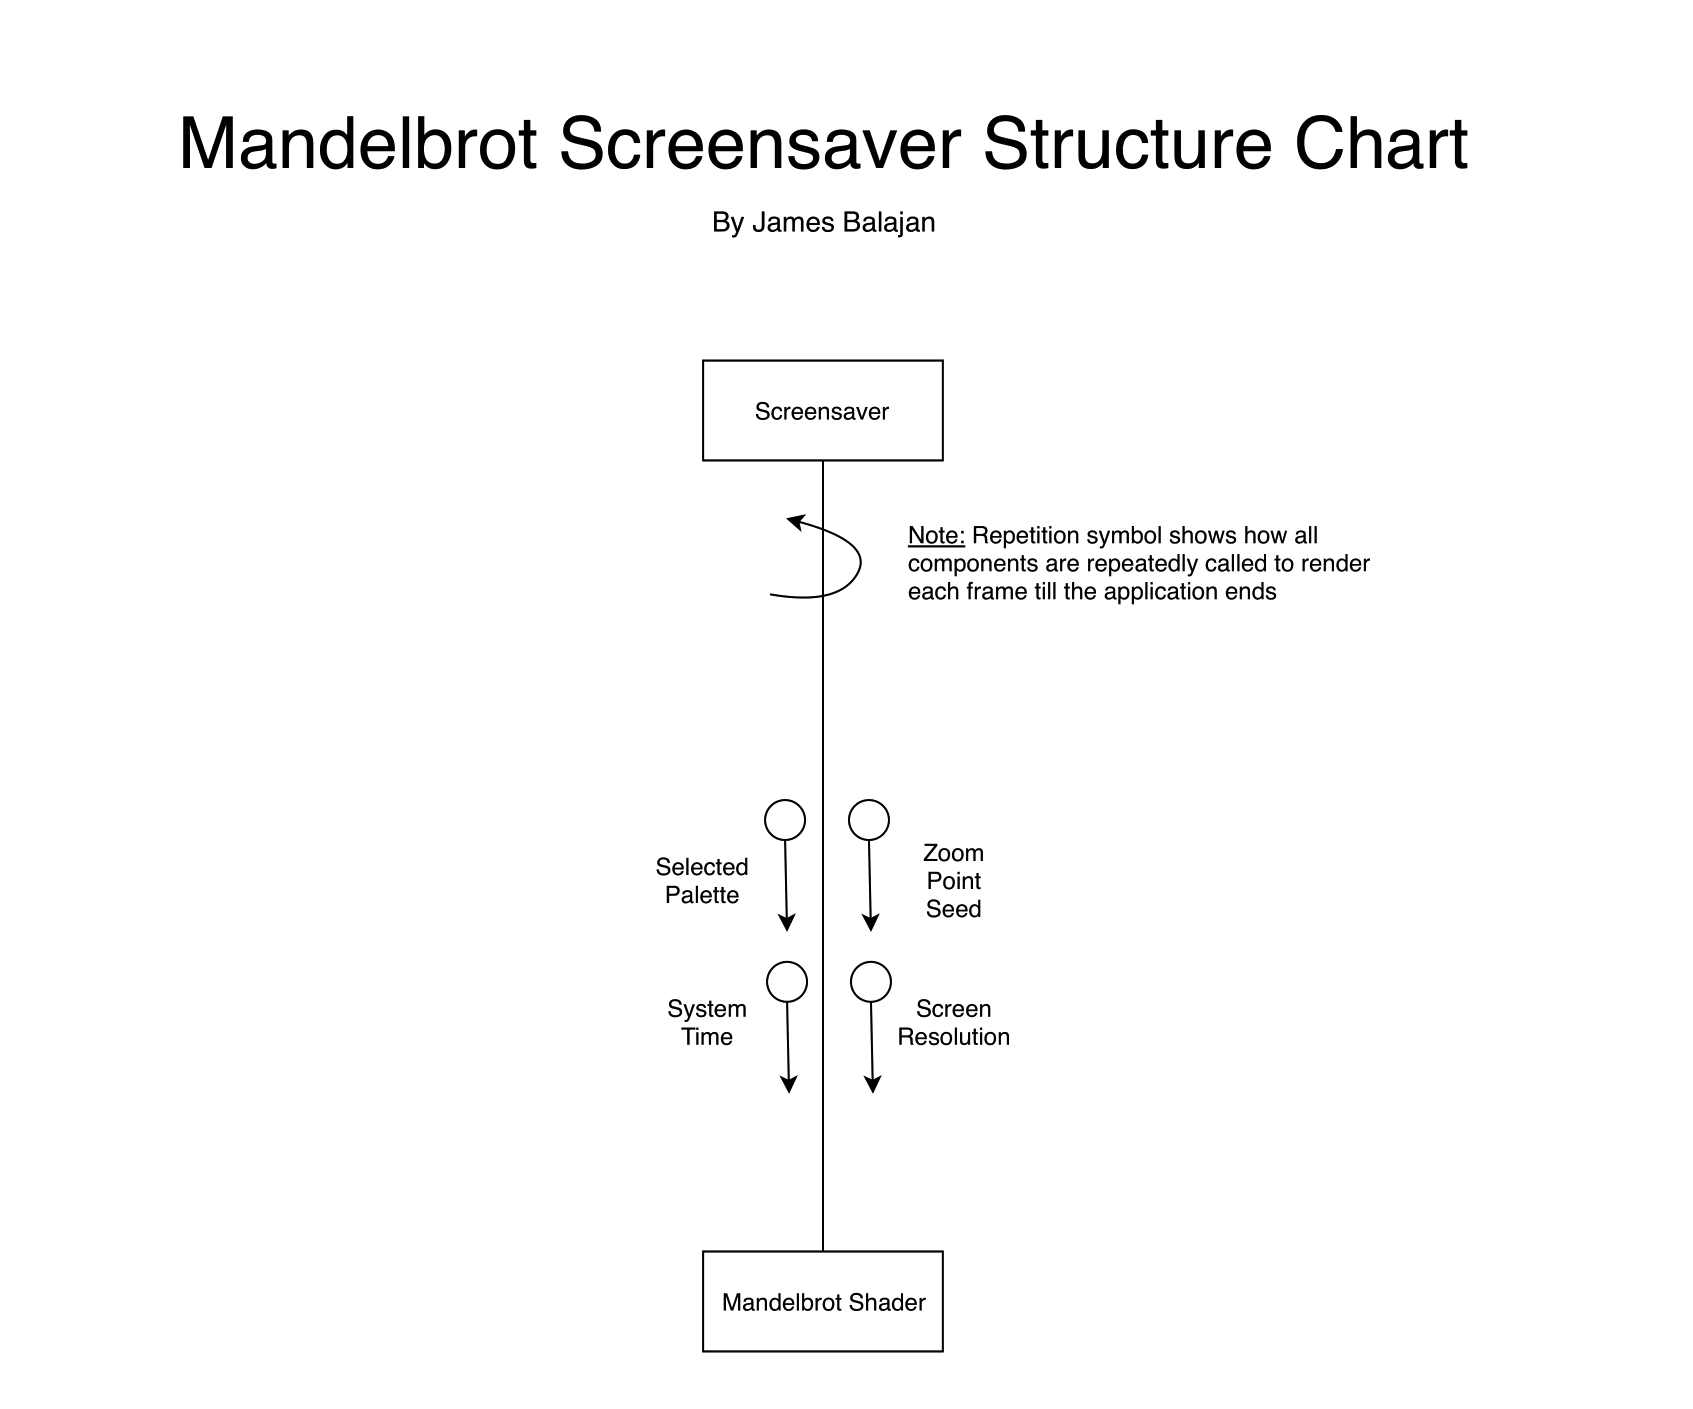
\includegraphics[width=1.0\linewidth]{Mandelbrot Screensaver Structure Chart}
	\caption{Mandelbrot Screensaver Structure Chart}
	\label{app:mandelbrot-struc}
\end{figure}
\newpage

\subsection{Mandelbrot Screensaver Storyboard}
\begin{figure}[H]
	\centering
	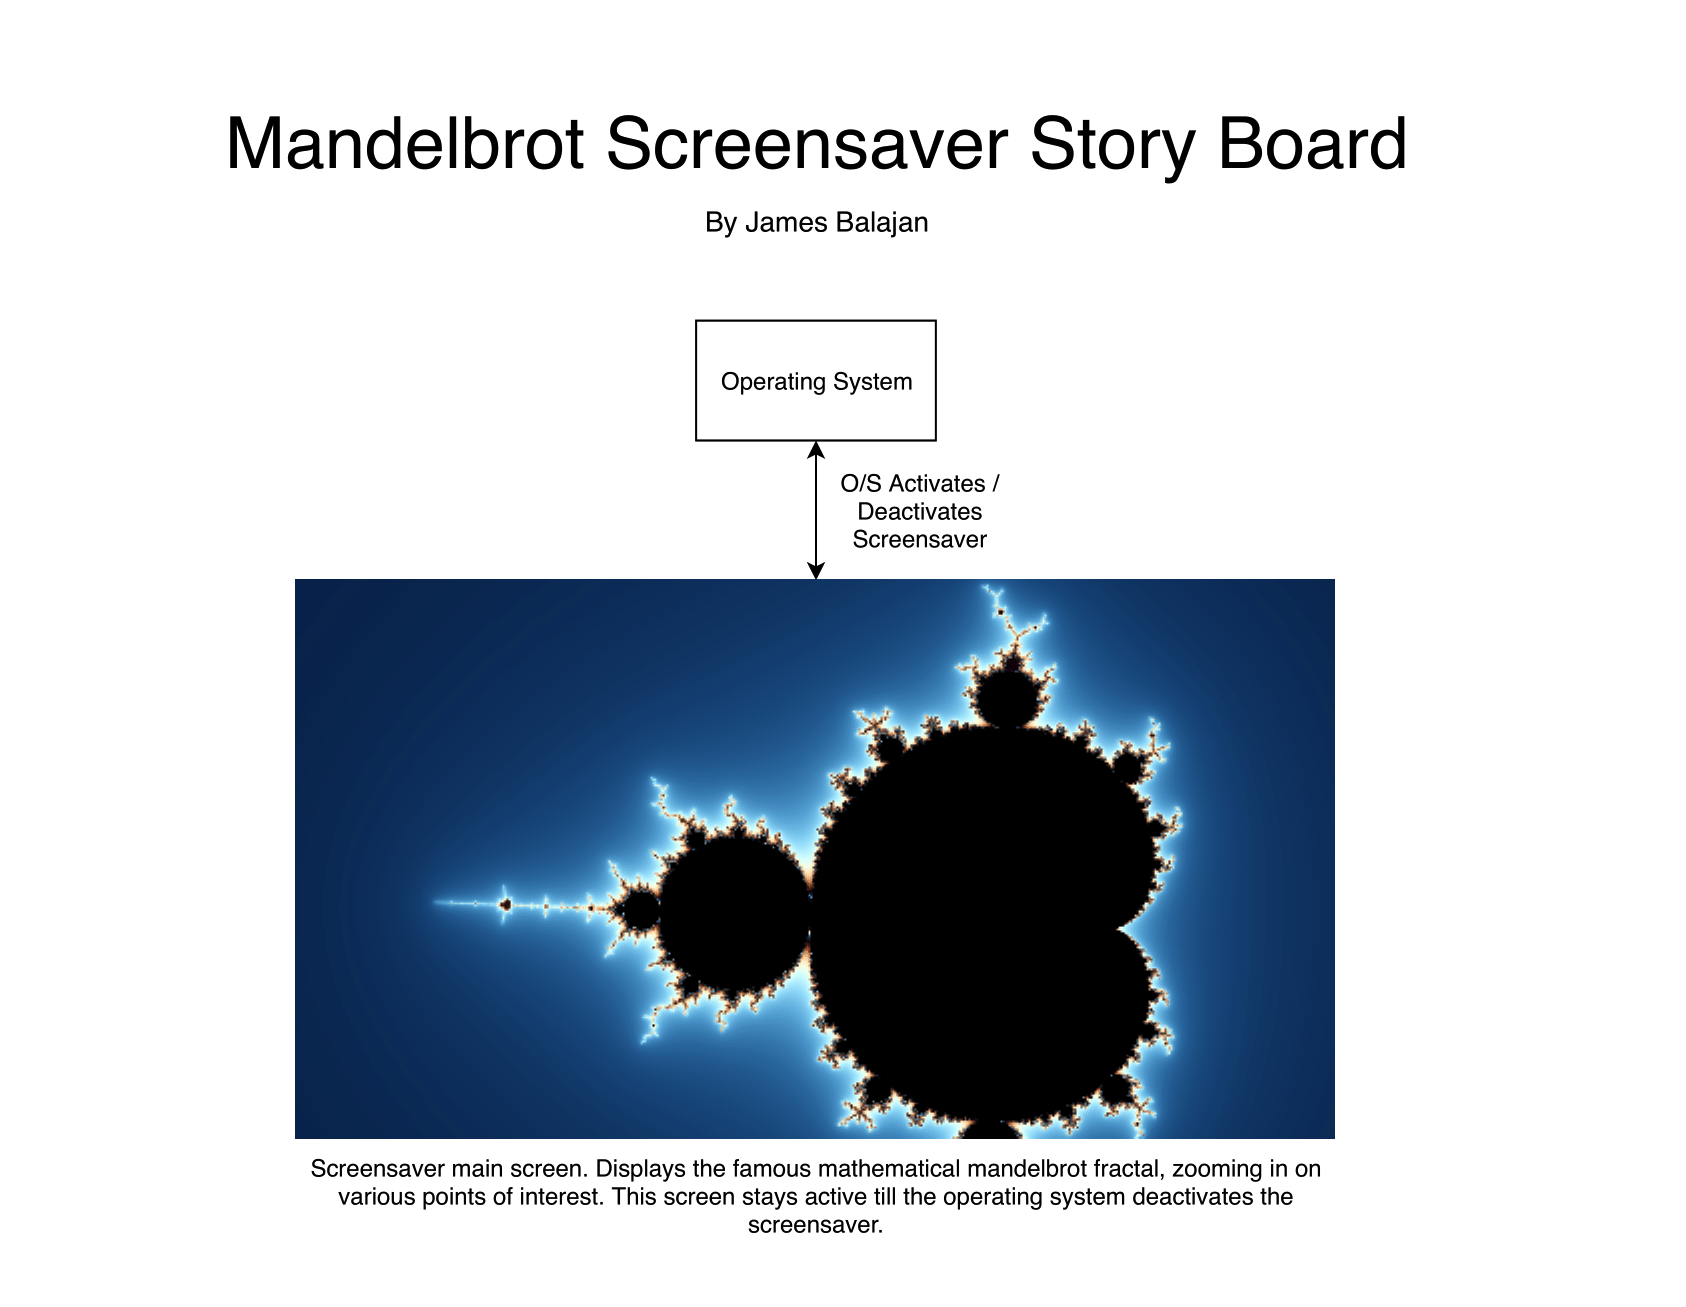
\includegraphics[width=1.0\linewidth]{Mandelbrot Screensaver Story Board}
	\caption{Mandelbrot Screensaver Storyboard}
	\label{app:mandelbrot-story}
\end{figure}
\newpage

\subsection{Metaballs Screensaver Context Diagram}
\begin{figure}[H]
	\centering
	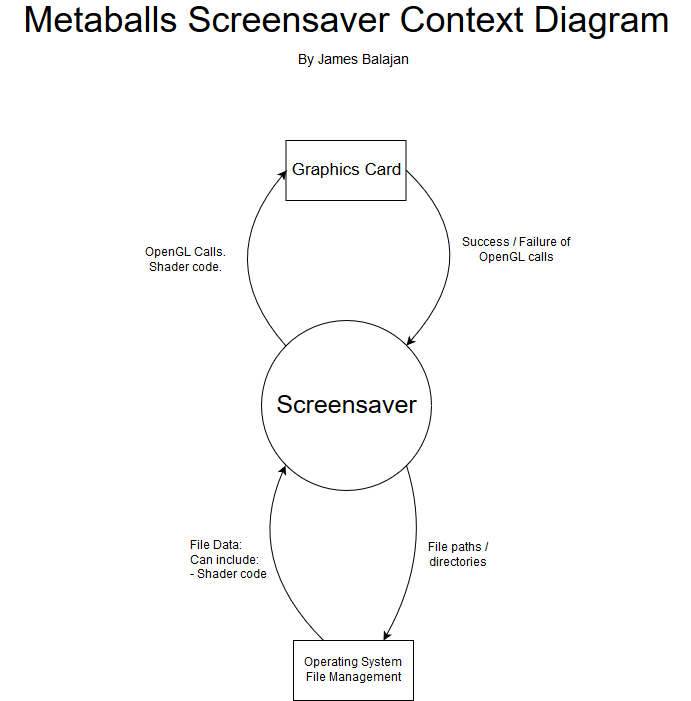
\includegraphics[width=1.0\linewidth]{Metaballs Screensaver Context Diagram}
	\caption{Metaballs Screensaver Context Diagram}
	\label{app:metaballs-context}
\end{figure}
\newpage

\subsection{Metaballs Screensaver Data Flow Diagram}
\begin{figure}[H]
	\centering
	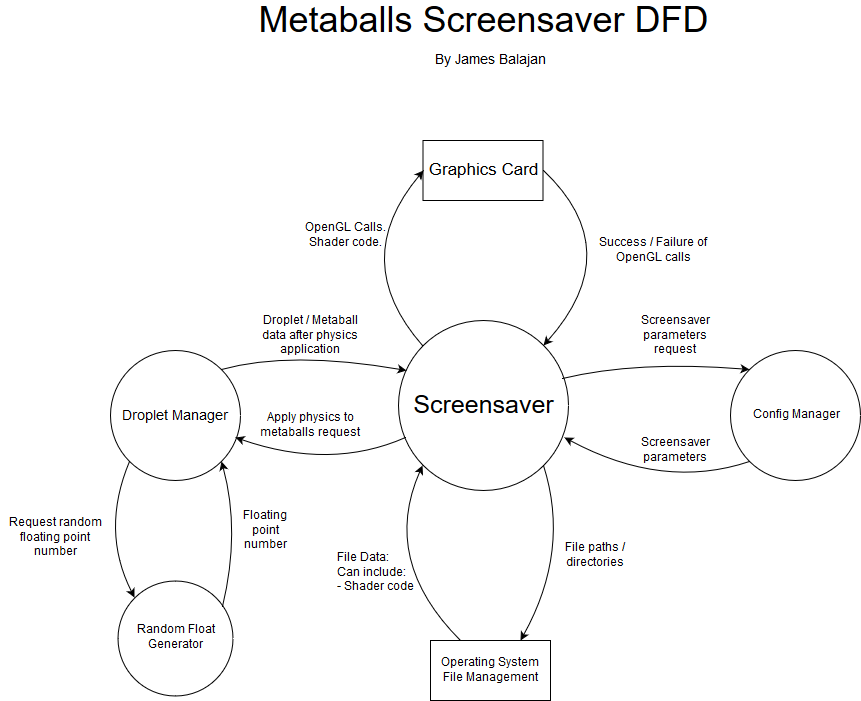
\includegraphics[width=1.0\linewidth]{Metaballs Screensaver DFD}
	\caption{Metaballs Screensaver Data Flow Diagram}
	\label{app:metaballs-dfd}
\end{figure}
\newpage

\subsection{Metaballs Screensaver Structure Chart}
\begin{figure}[H]
	\centering
	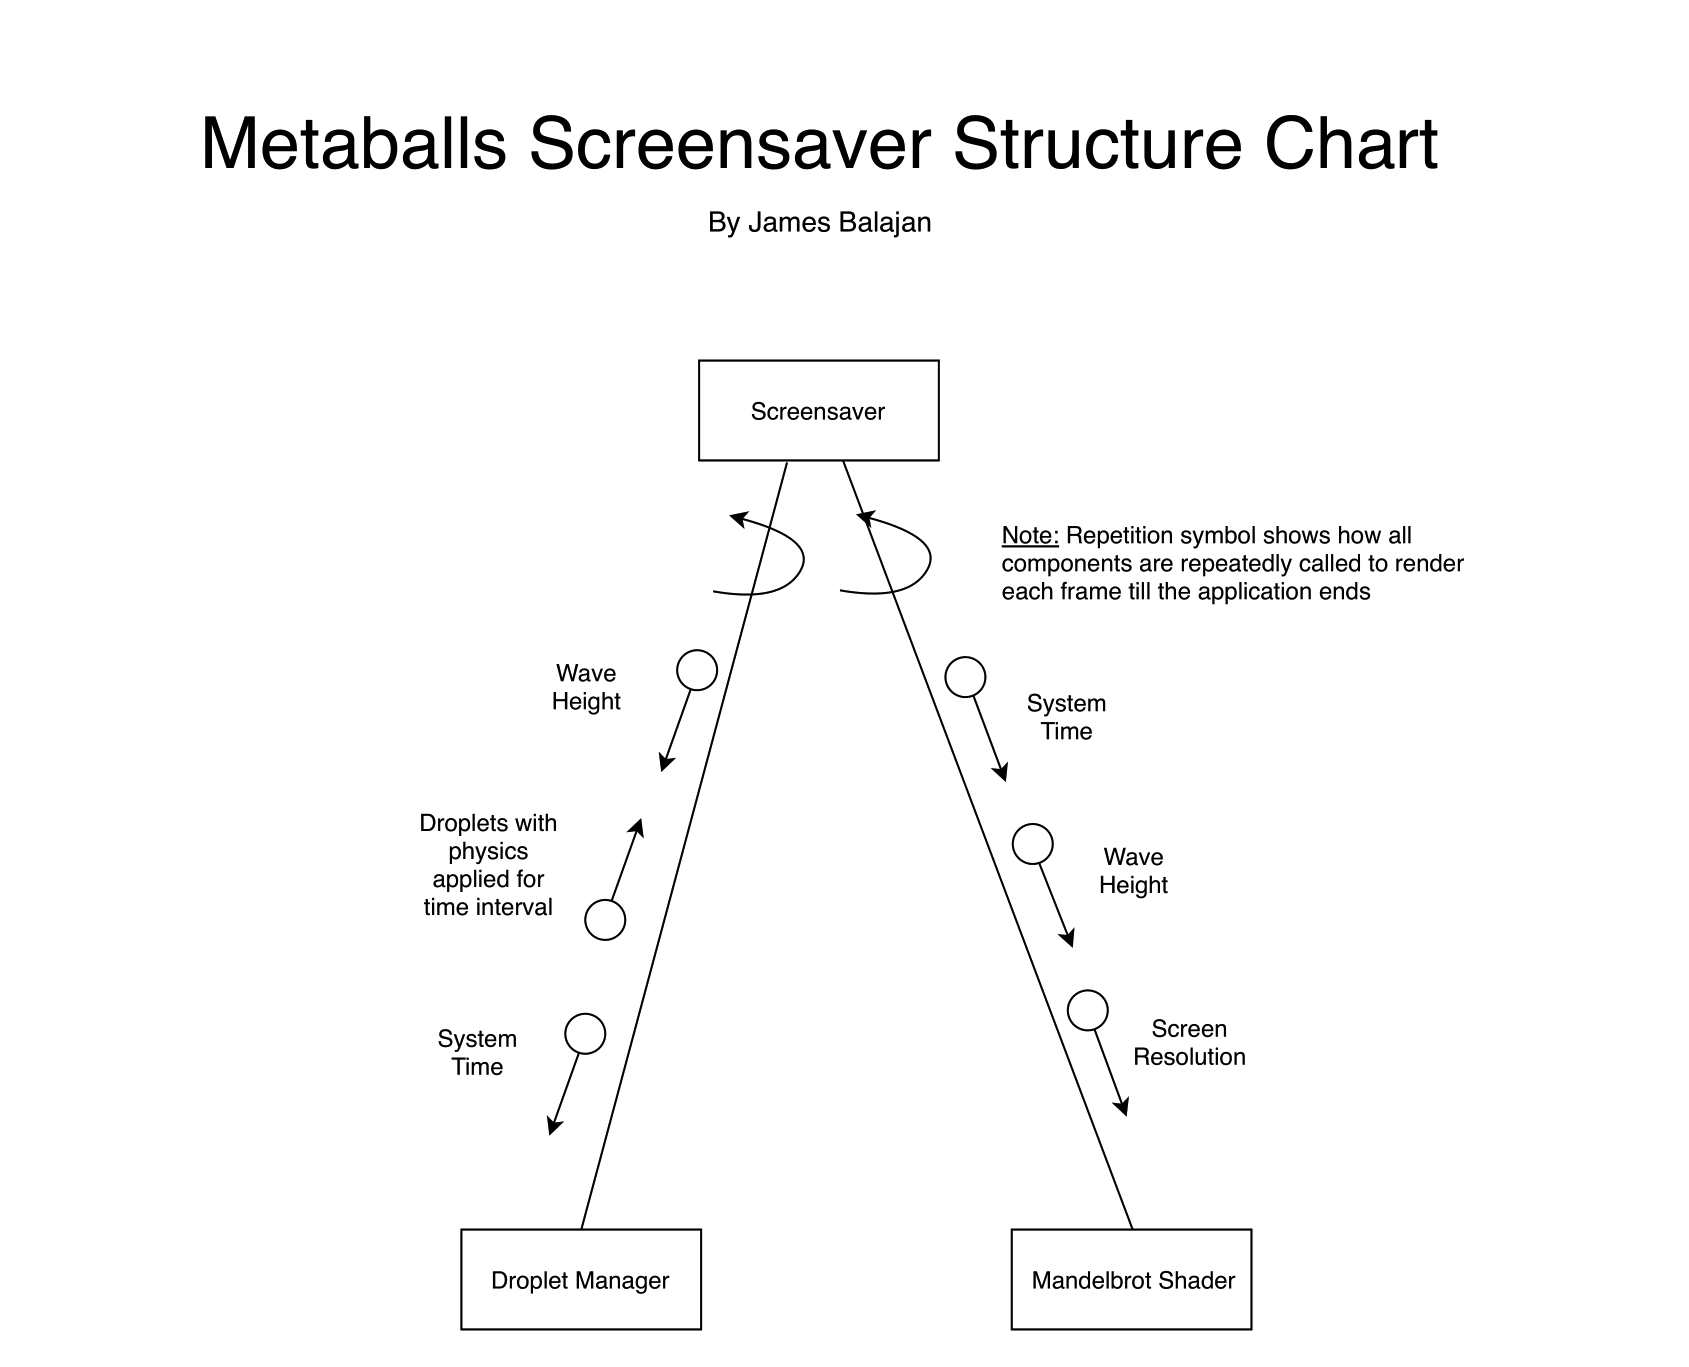
\includegraphics[width=1.0\linewidth]{Metaballs Screensaver Structure Chart}
	\caption{Metaballs Screensaver Structure Chart}
	\label{app:metaballs-struc}
\end{figure}
\newpage

\subsection{Metaballs Screensaver Storyboard}
\begin{figure}[H]
	\centering
	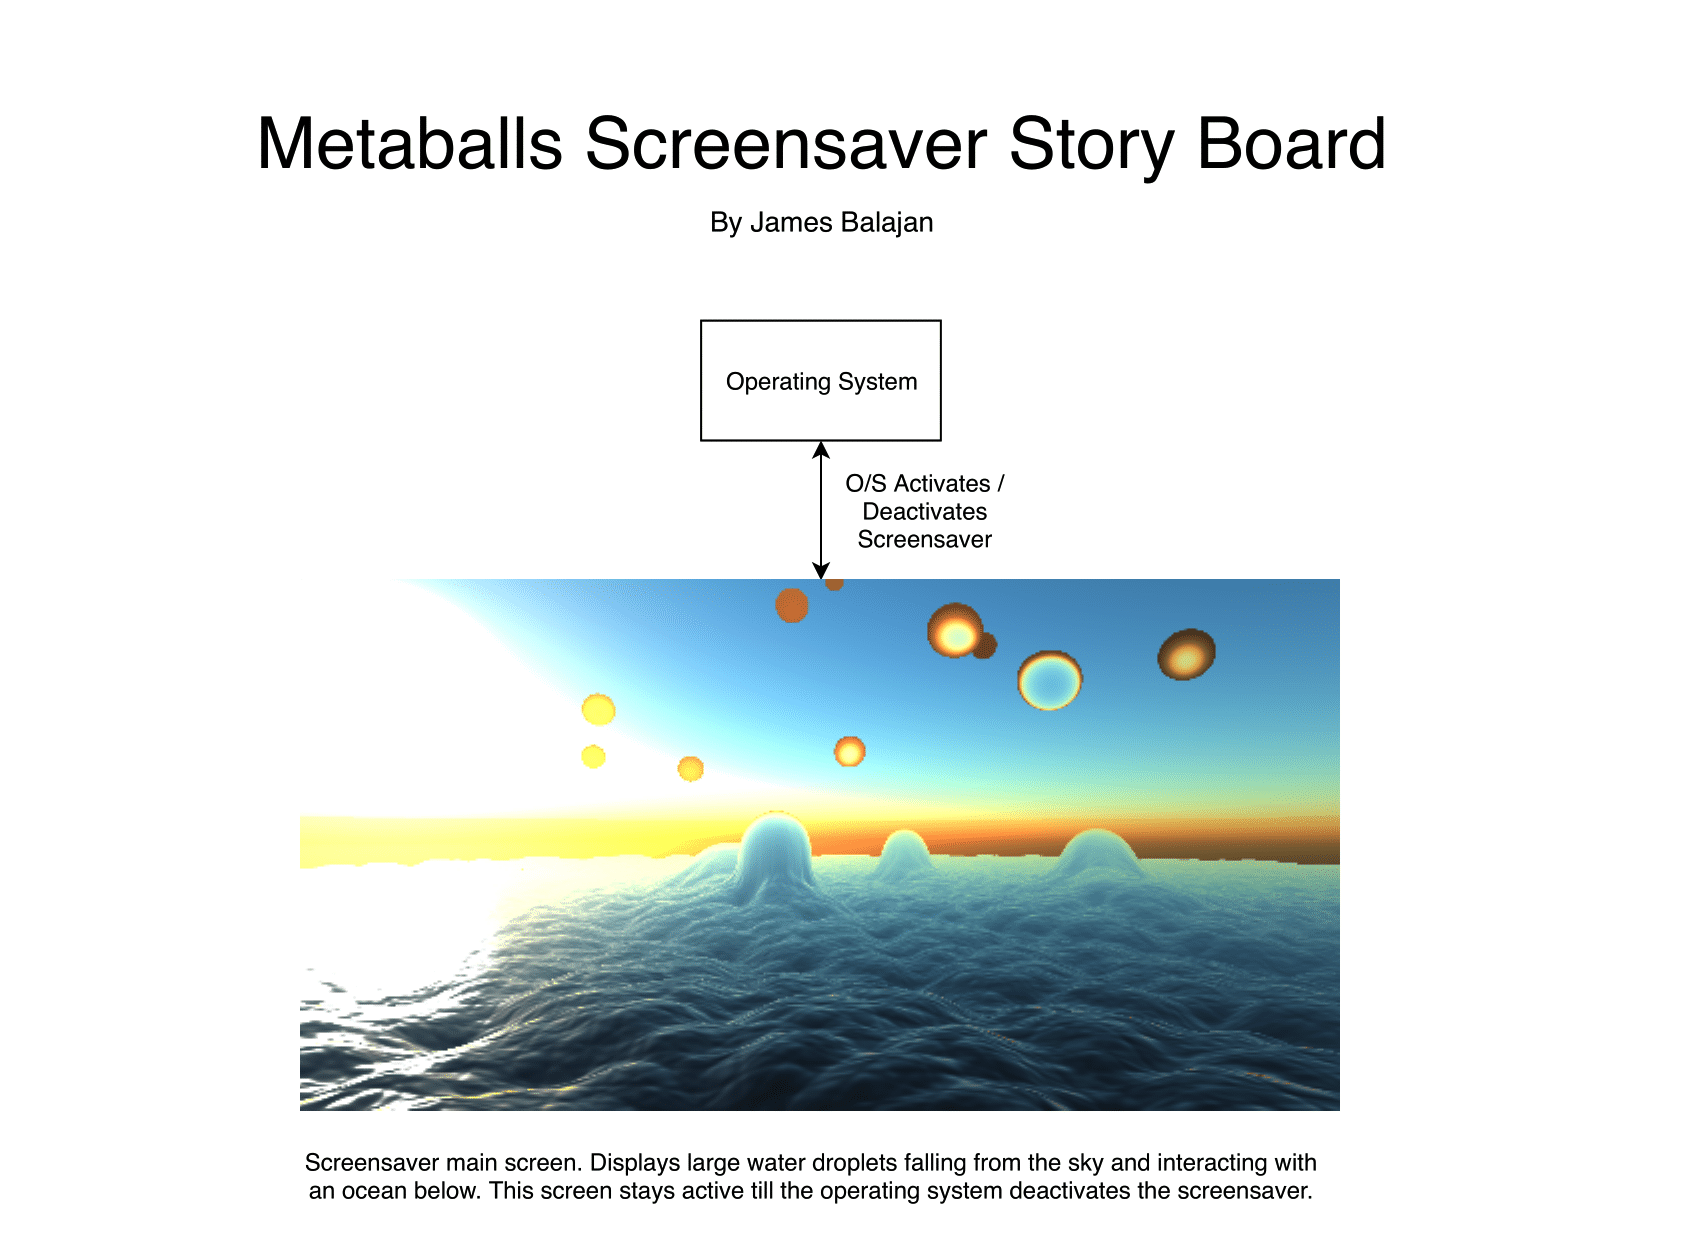
\includegraphics[width=1.0\linewidth]{Metaballs Screensaver Story Board}
	\caption{Metaballs Screensaver Storyboard}
	\label{app:metaballs-story}
\end{figure}
\newpage

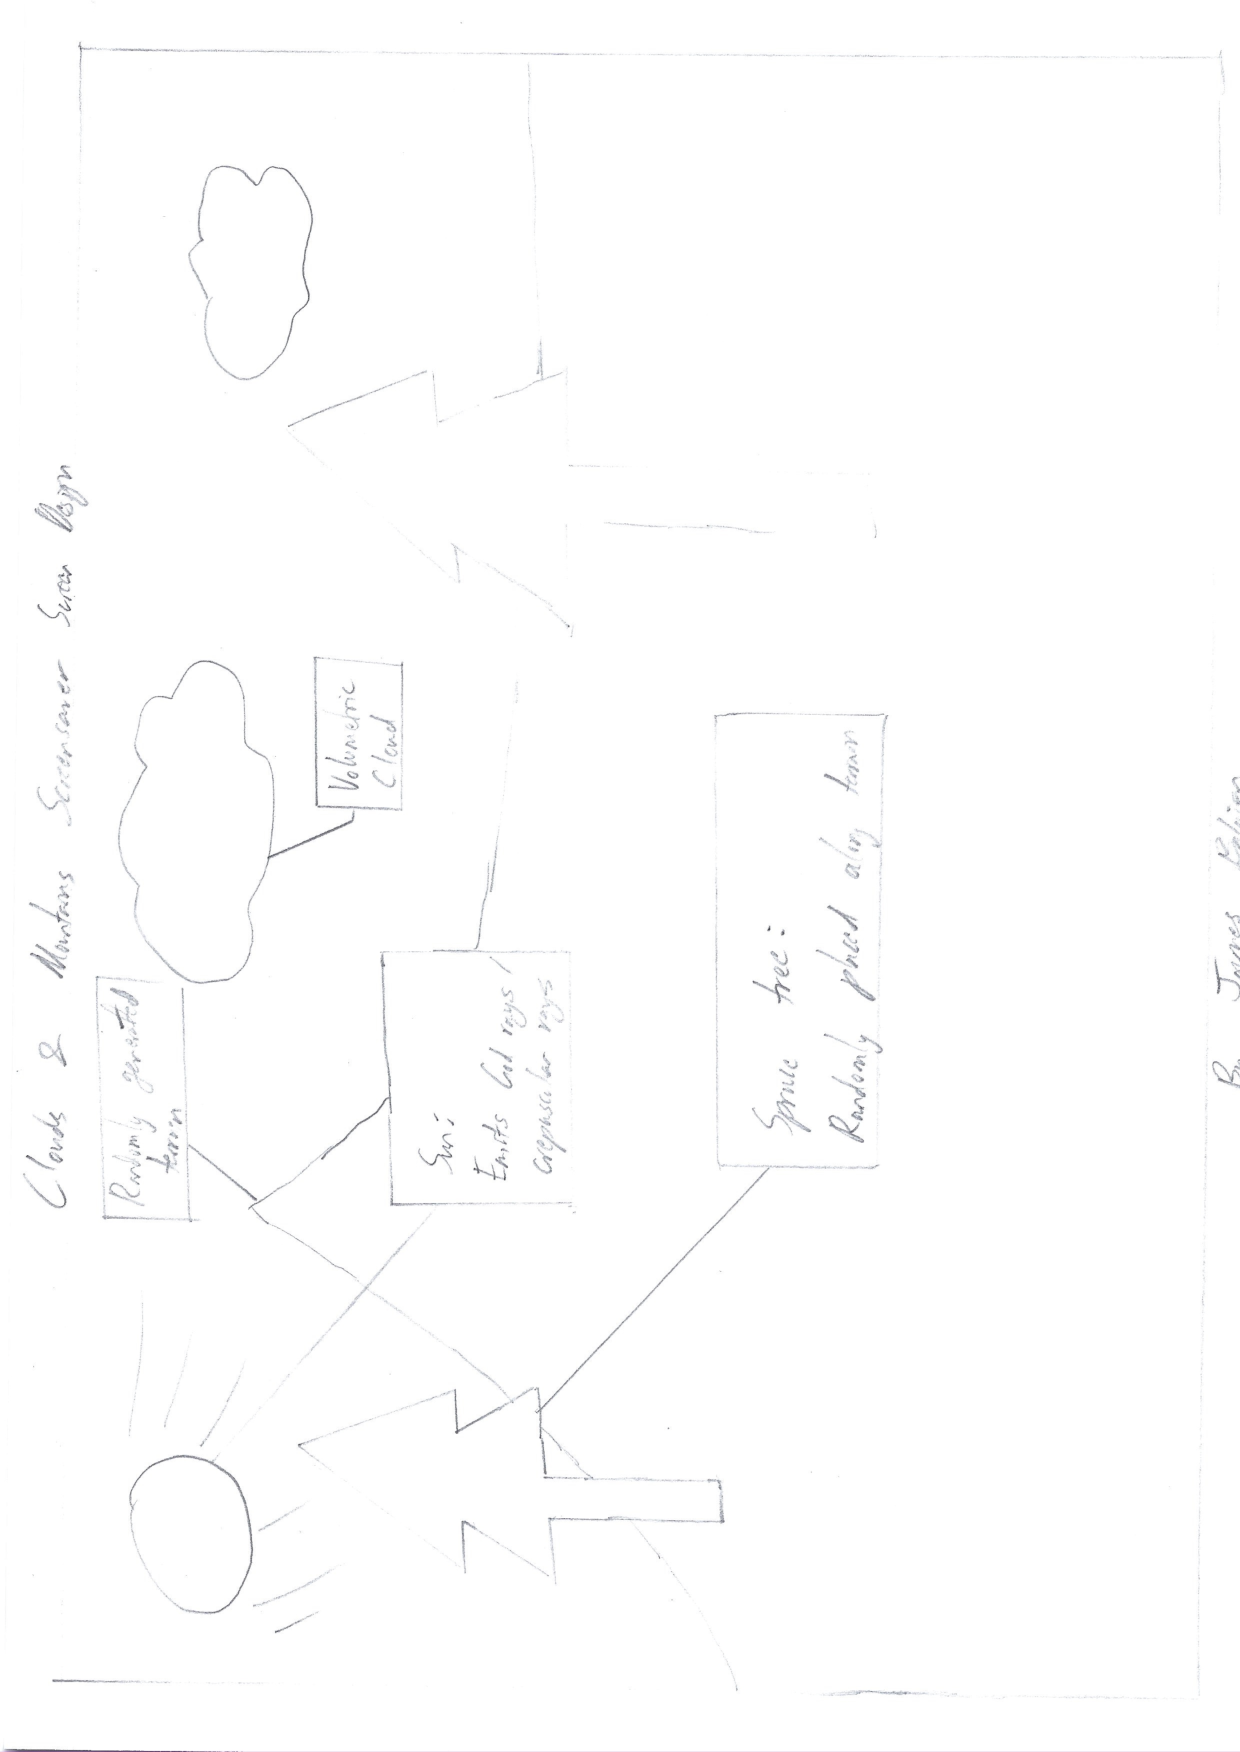
\includepdf[pages=1, scale=0.78, pagecommand={\subsection{Clouds and Mountains Screensaver Screen Design} \label{app:clouds-screen}}]{external-pdfs/CloudsAndMountainsScreen.pdf}
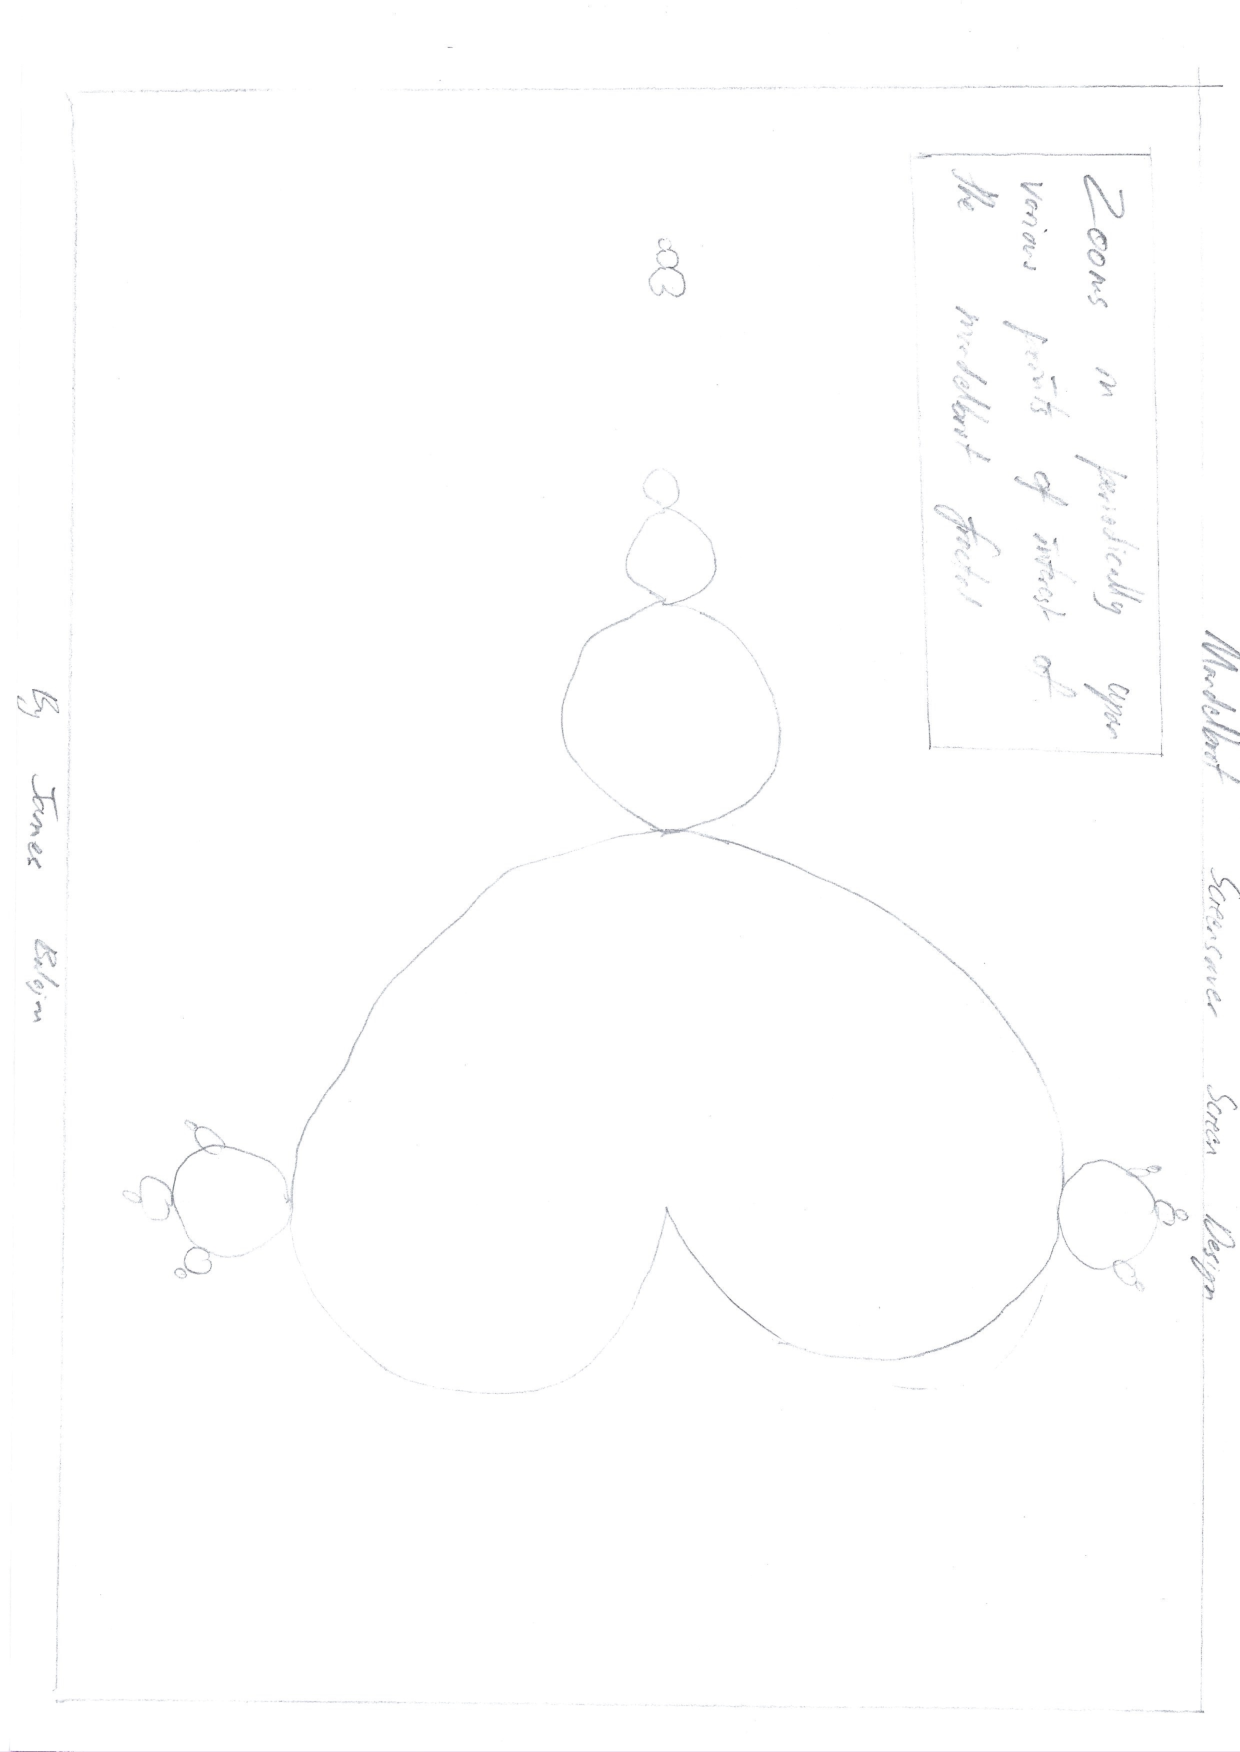
\includepdf[pages=1, scale=0.78, pagecommand={\subsection{Mandelbrot Screensaver Screen Design} \label{app:mandelbrot-screen}}]{external-pdfs/MandelbrotScreen.pdf}
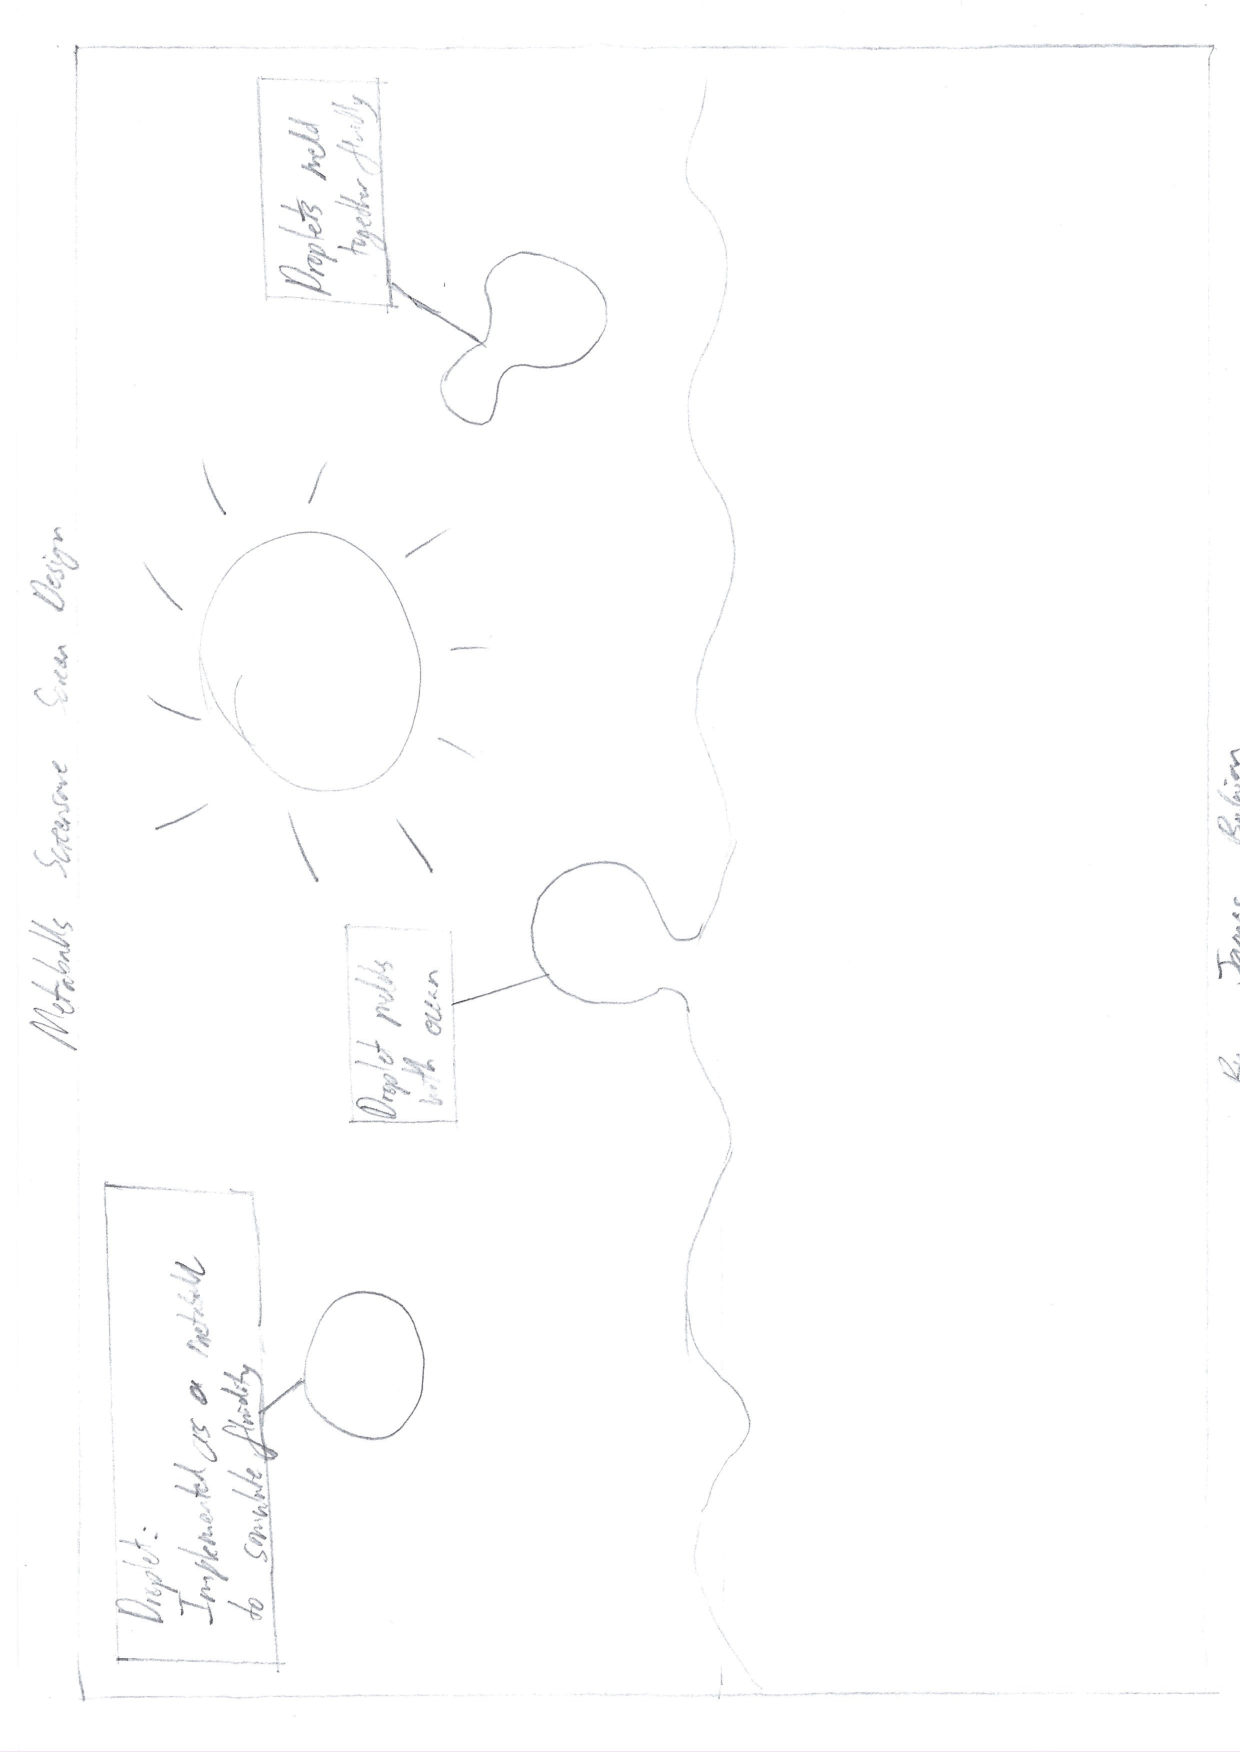
\includepdf[pages=1, scale=0.78, pagecommand={\subsection{Metaballs Screensaver Screen Design} \label{app:metaballs-screen}}]{external-pdfs/MetaballsScreen.pdf}

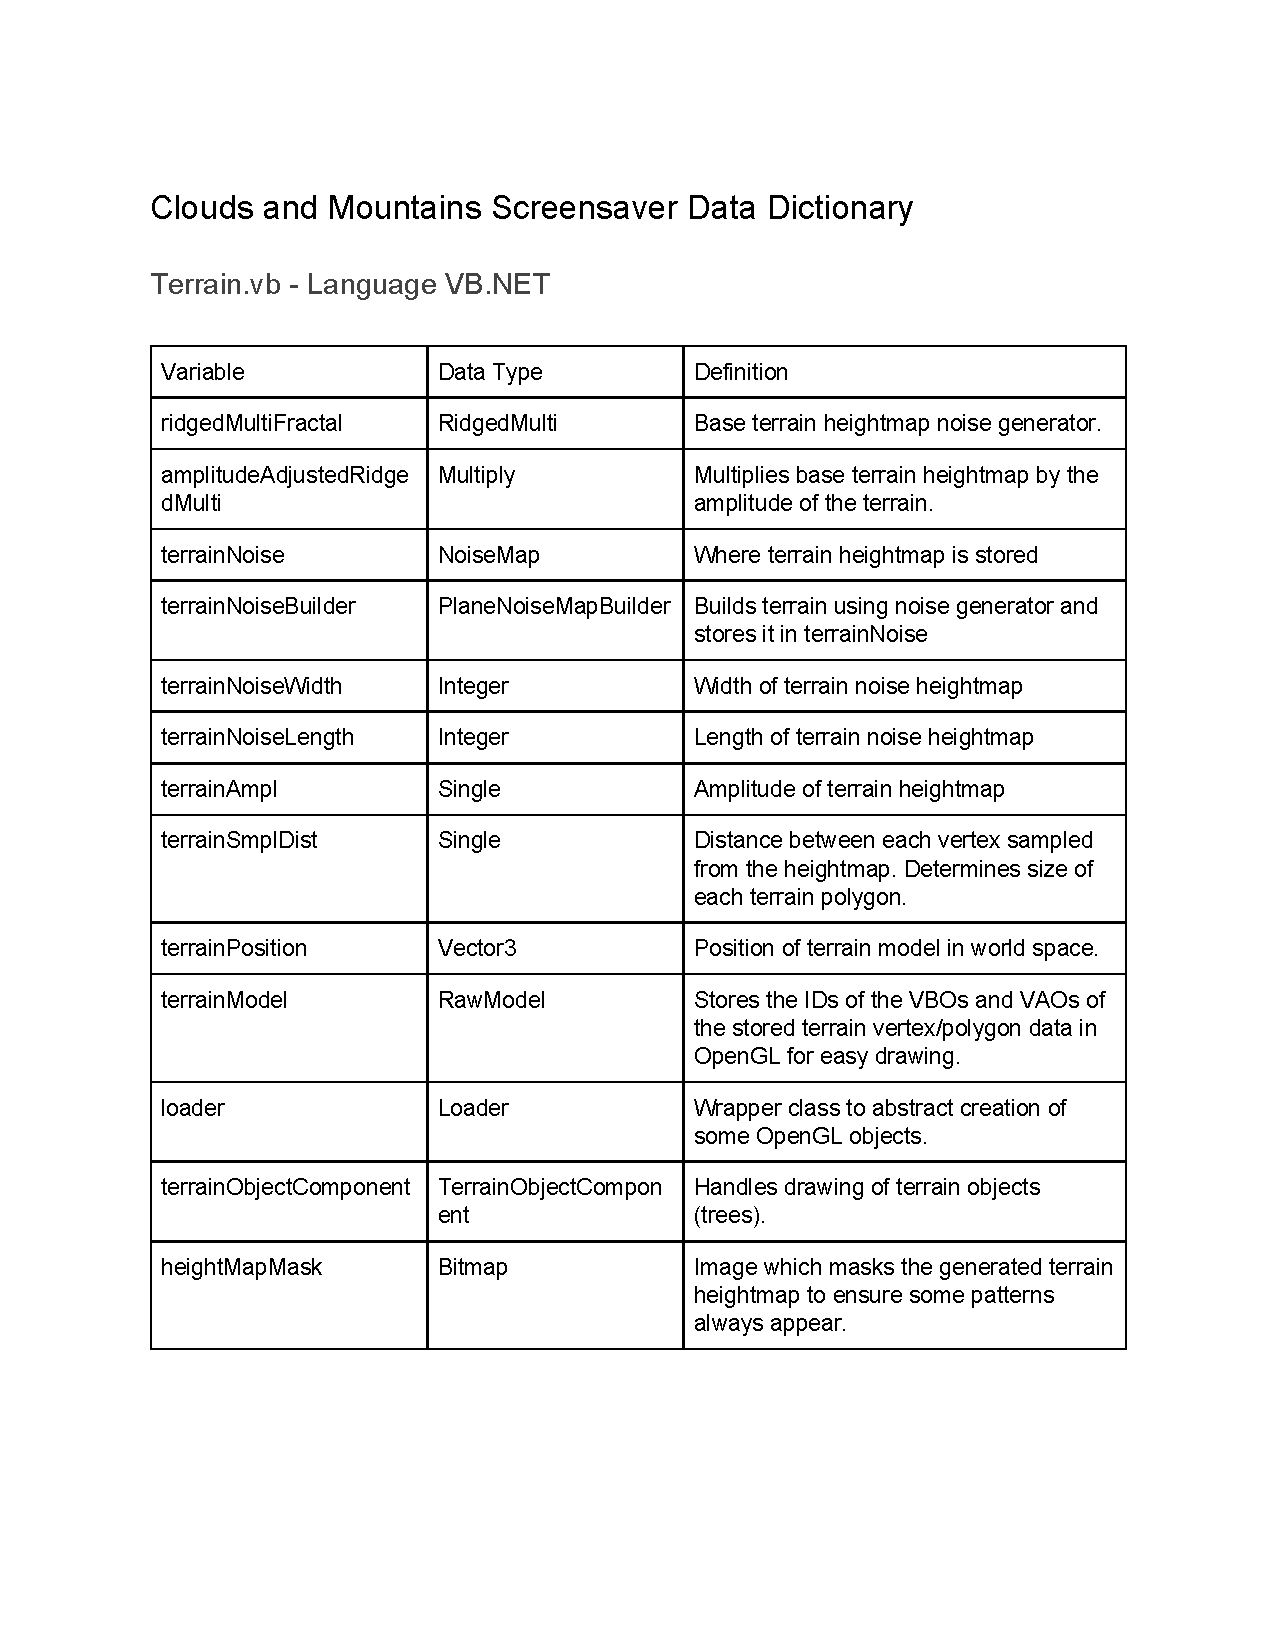
\includepdf[pages=1, scale=0.9, pagecommand={\subsection{Data Dictionary} \label{app:data-dictionary}}]{external-pdfs/SDDDataDictionary.pdf}
\includepdf[pages={2-}, scale=0.9, pagecommand={}]{external-pdfs/SDDDataDictionary.pdf}

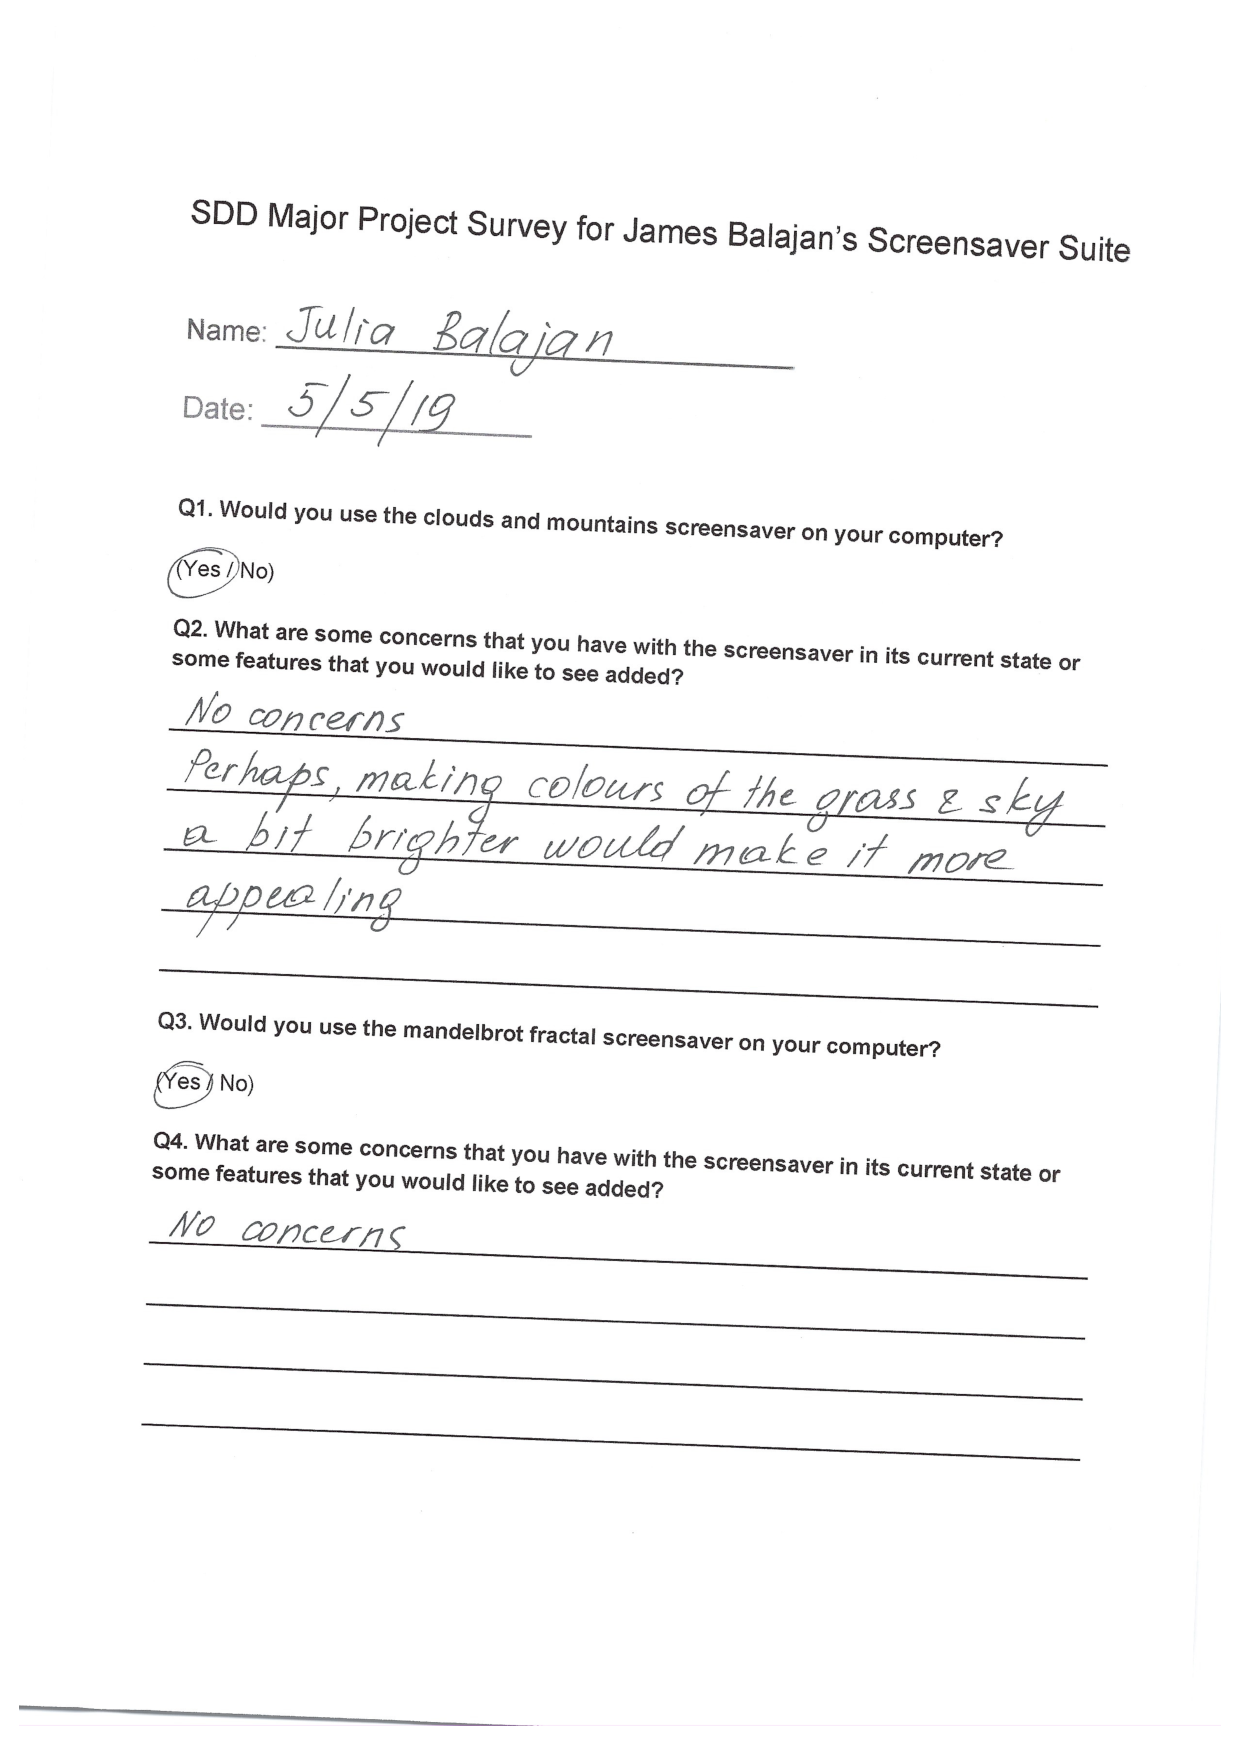
\includepdf[pages=1, scale=0.78, pagecommand={\section{Survey Responses} \subsection{Julia Balajan - Survey Response} \label{app:survey-julia}}]{external-pdfs/JuliaBalajan.pdf}
\includepdf[pages=2, scale=0.78, pagecommand={}]{external-pdfs/JuliaBalajan.pdf}

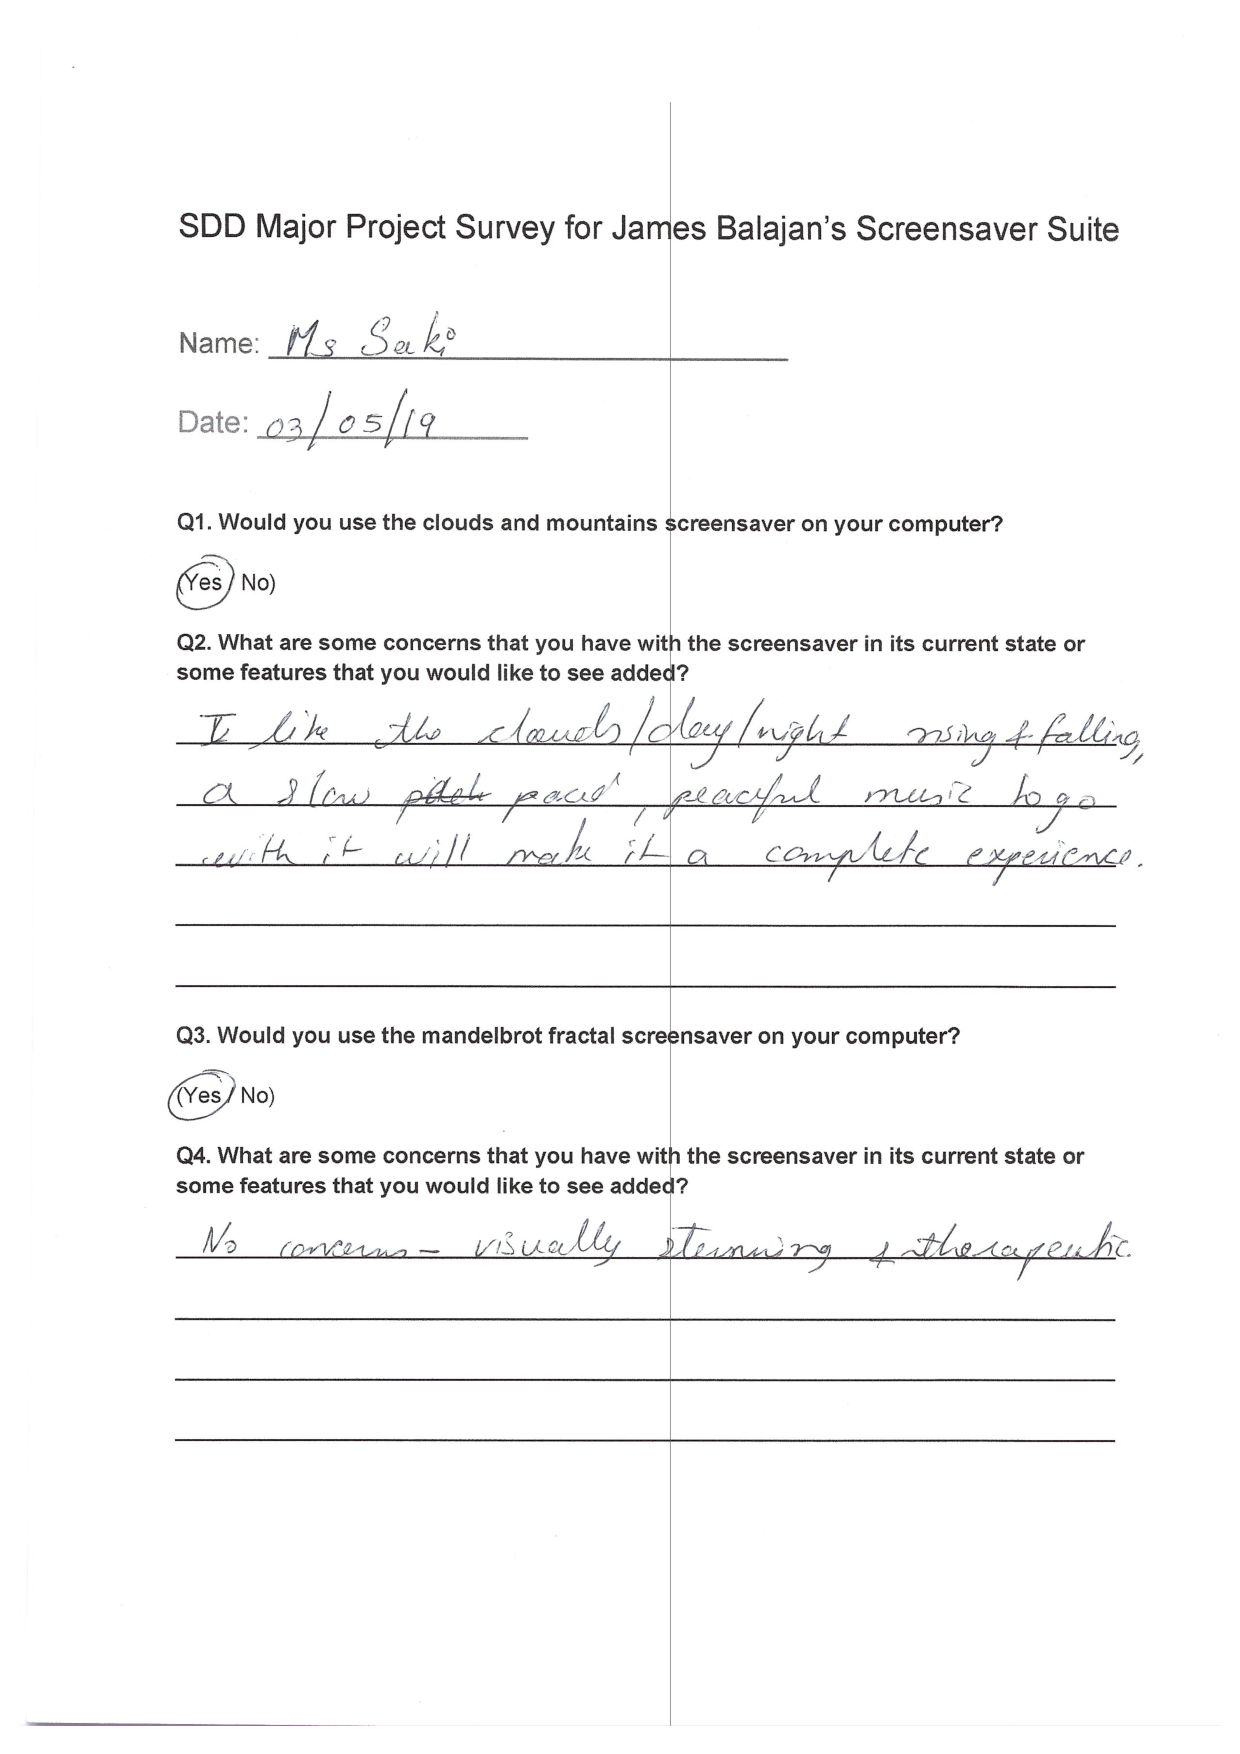
\includepdf[pages=1, scale=0.78, pagecommand={\subsection{Ms Saki - Survey Response} \label{app:survey-aartee}}]{external-pdfs/AarteeSaki.pdf}
\includepdf[pages=2, scale=0.78, pagecommand={}]{external-pdfs/AarteeSaki.pdf}

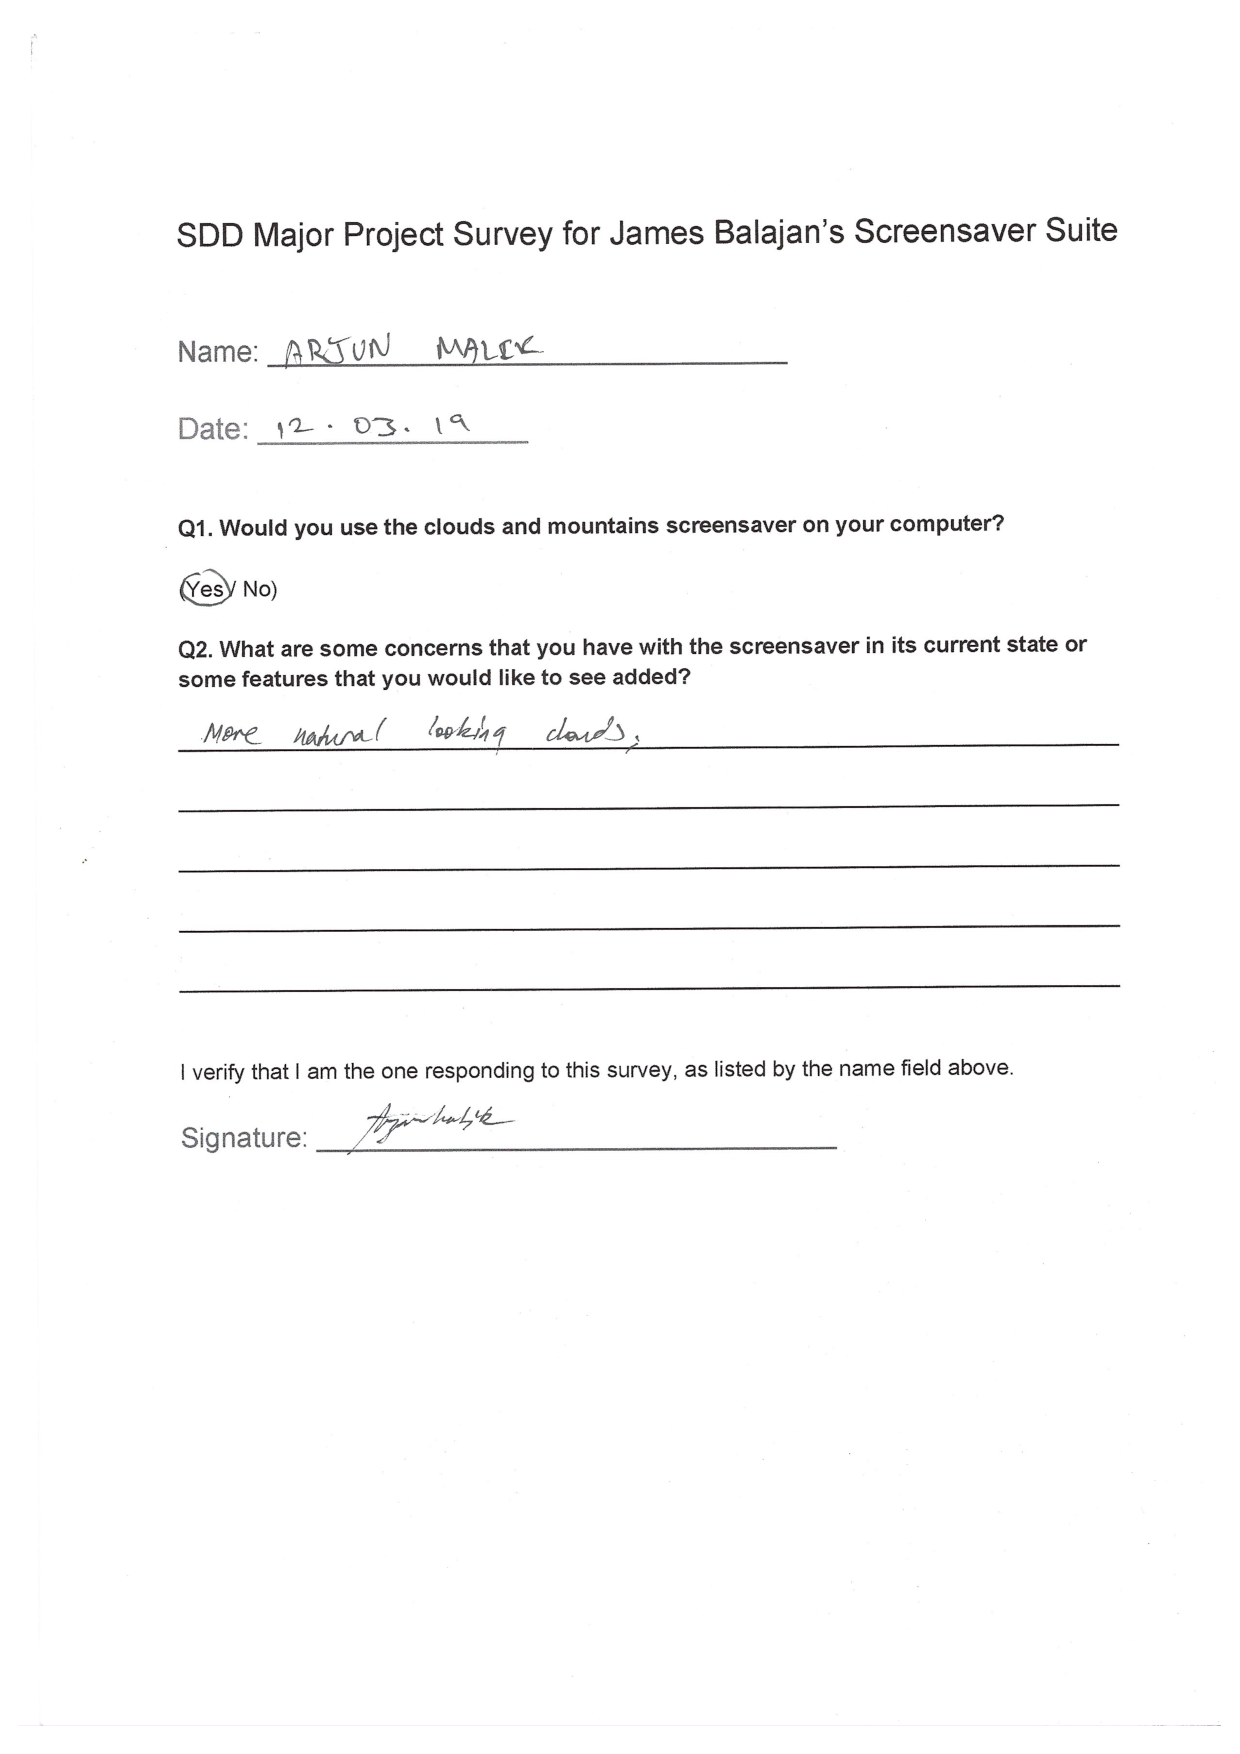
\includepdf[pages=1, scale=0.78, pagecommand={\subsection{Arjun Malik - Survey Response 1} \label{app:survey-arjun-1}}]{external-pdfs/ArjunMalikOld.pdf}
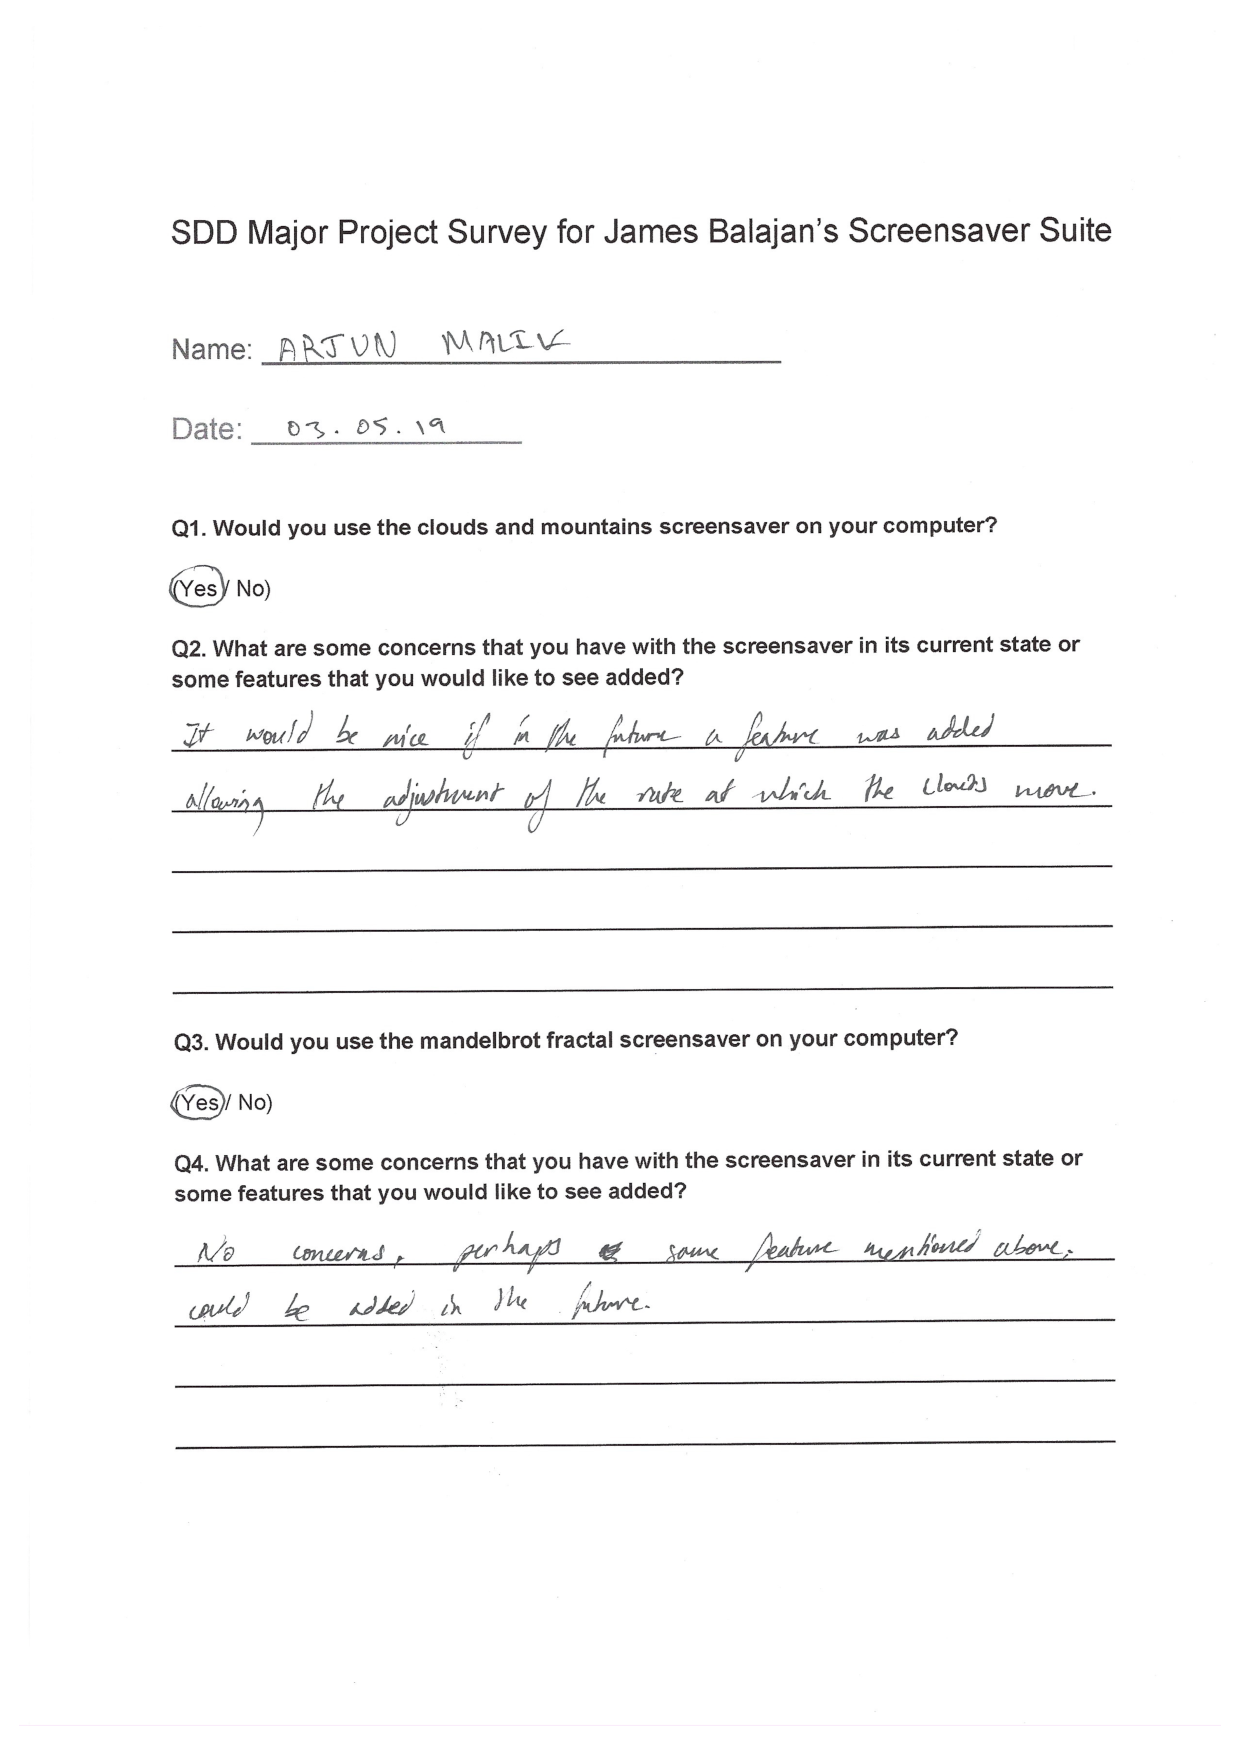
\includepdf[pages=1, scale=0.78, pagecommand={\subsection{Arjun Malik - Survey Response 2} \label{app:survey-arjun-2}}]{external-pdfs/ArjunMalik.pdf}
\includepdf[pages=2, scale=0.78, pagecommand={}]{external-pdfs/ArjunMalik.pdf}

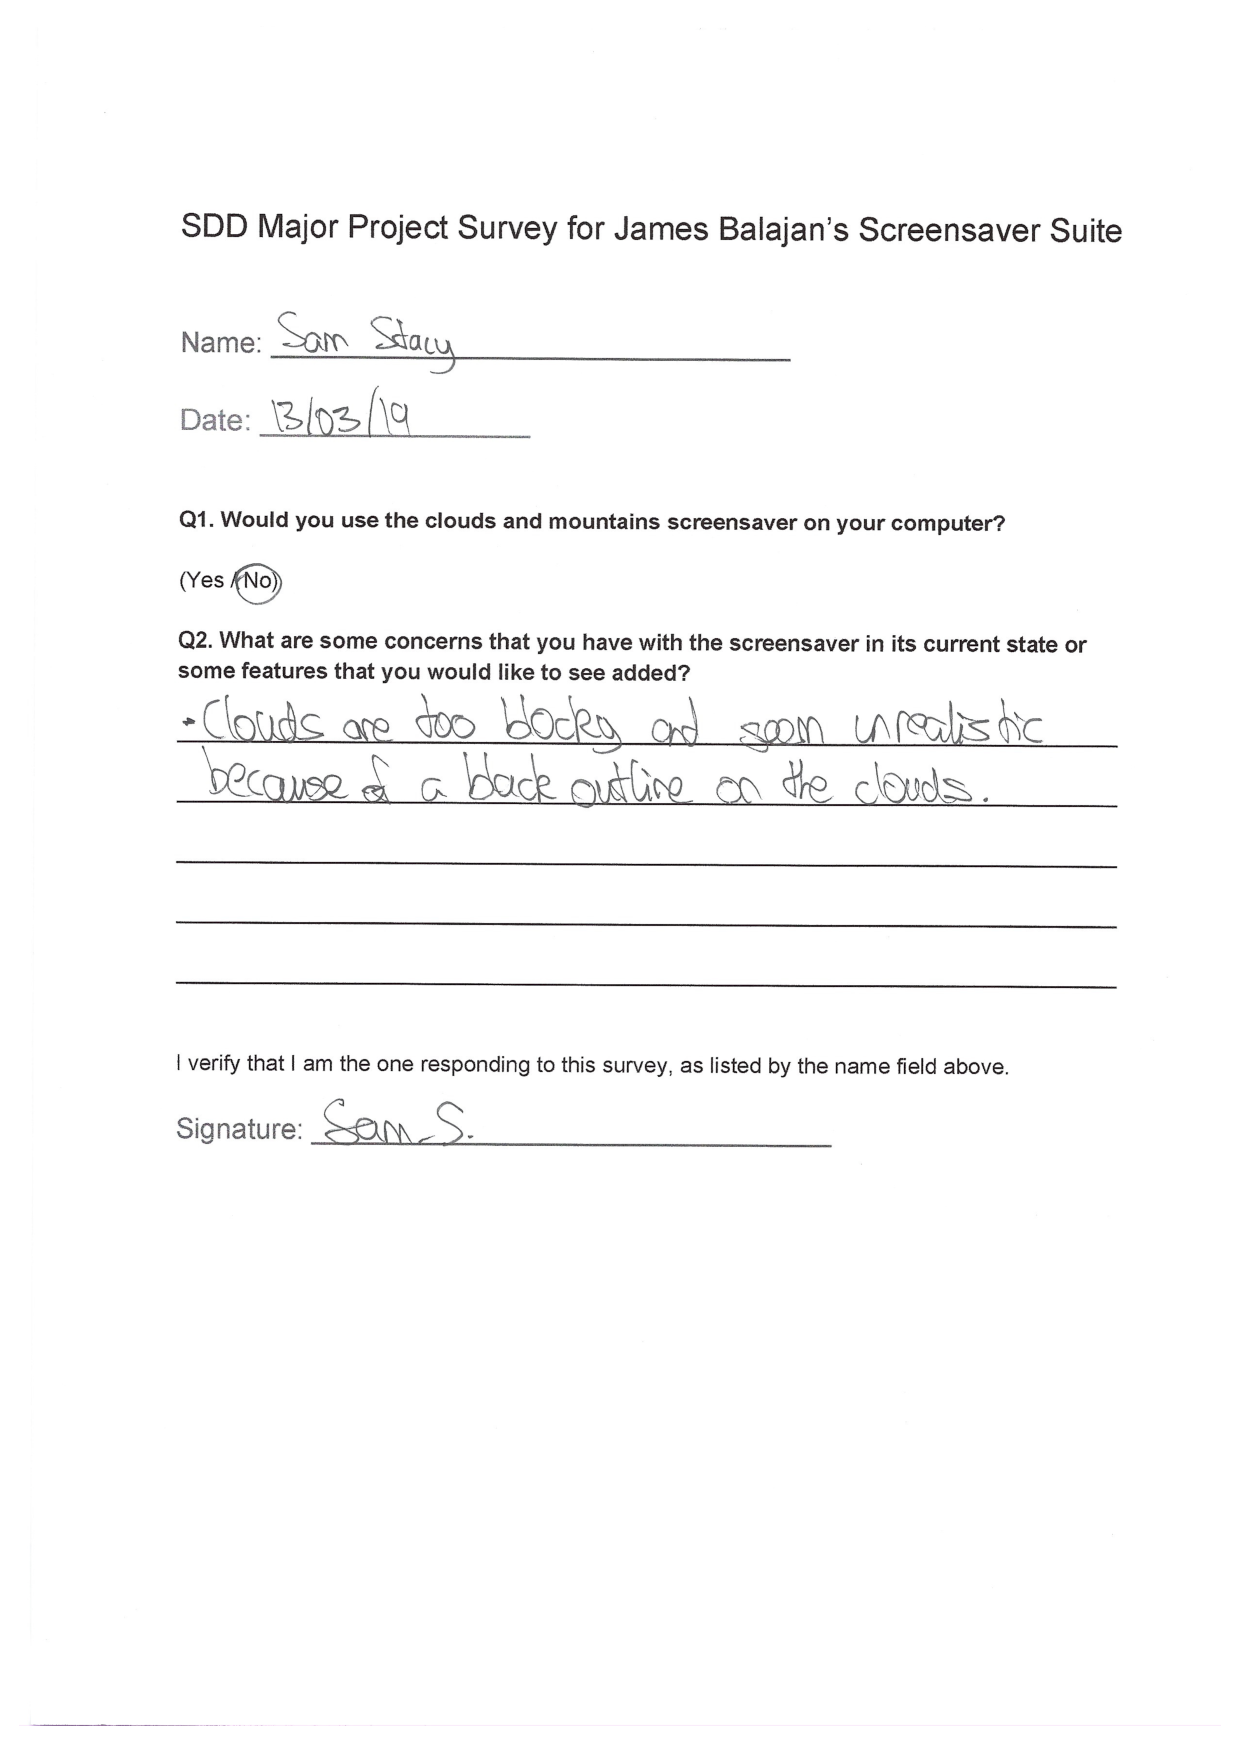
\includepdf[pages=1, scale=0.78, pagecommand={\subsection{Samuel Stacy - Survey Response 1} \label{app:survey-sam-1}}]{external-pdfs/SamStacyOld.pdf}
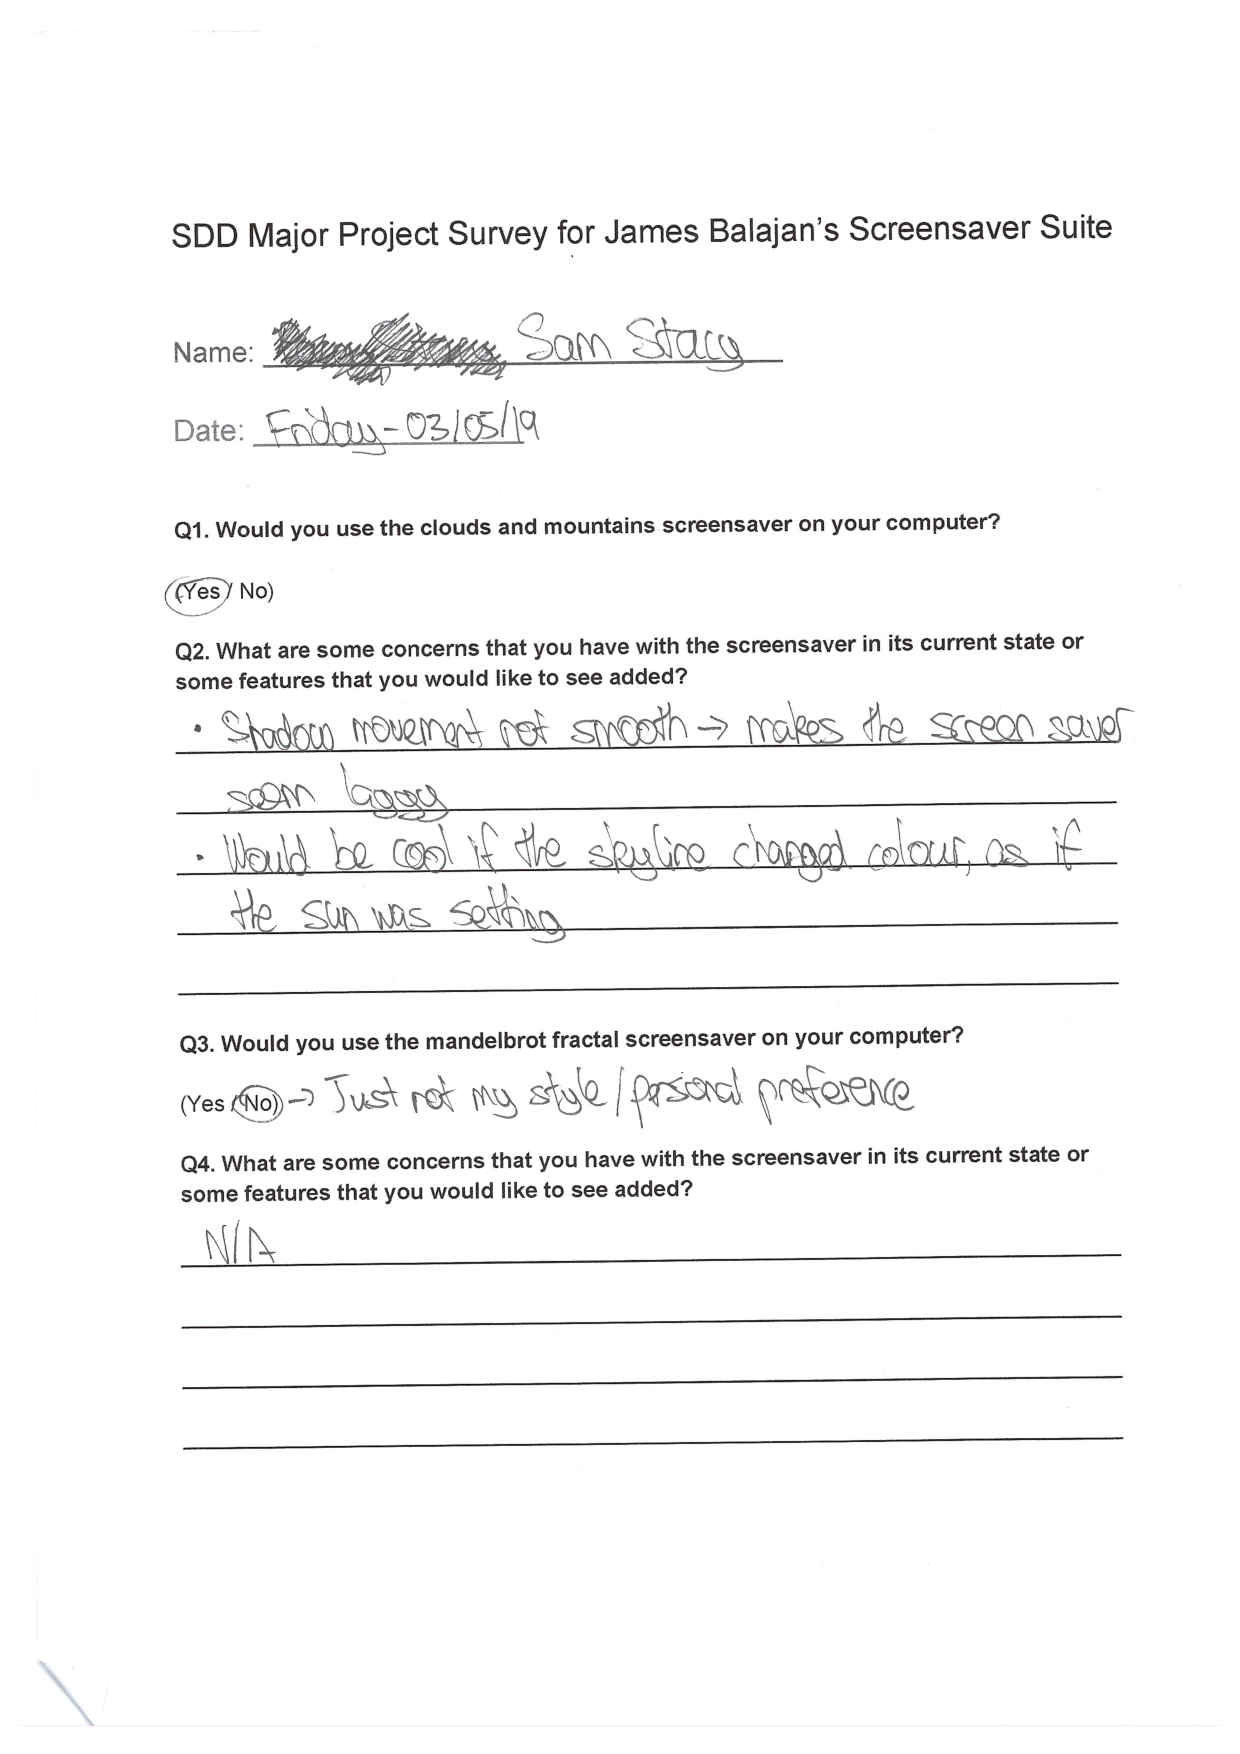
\includepdf[pages=1, scale=0.78, pagecommand={\subsection{Samuel Stacy - Survey Response 2} \label{app:survey-sam-2}}]{external-pdfs/SamStacy.pdf}
\includepdf[pages=2, scale=0.78, pagecommand={}]{external-pdfs/SamStacy.pdf}

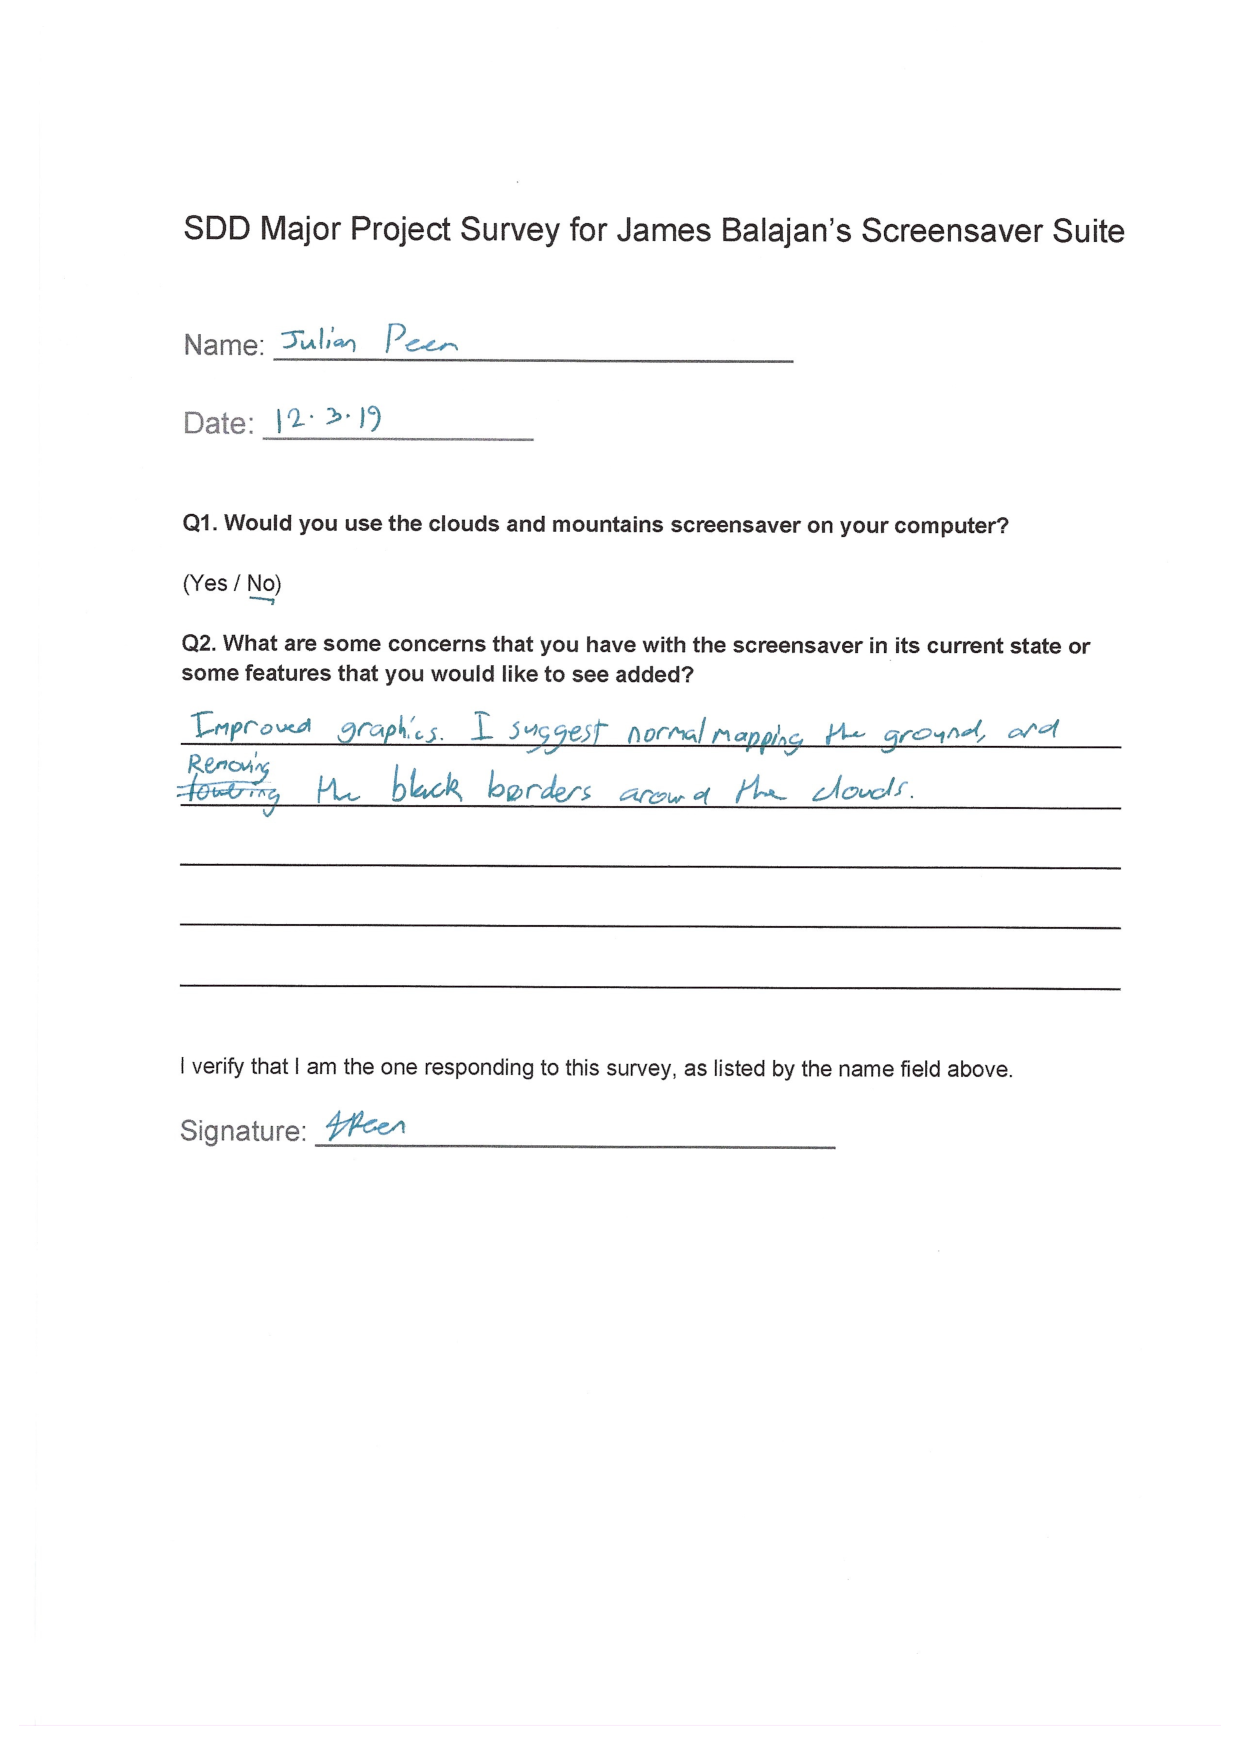
\includepdf[pages=1, scale=0.78, pagecommand={\subsection{Julian Peen - Survey Response 1} \label{app:survey-julian-1}}]{external-pdfs/JulianPeenOld.pdf}
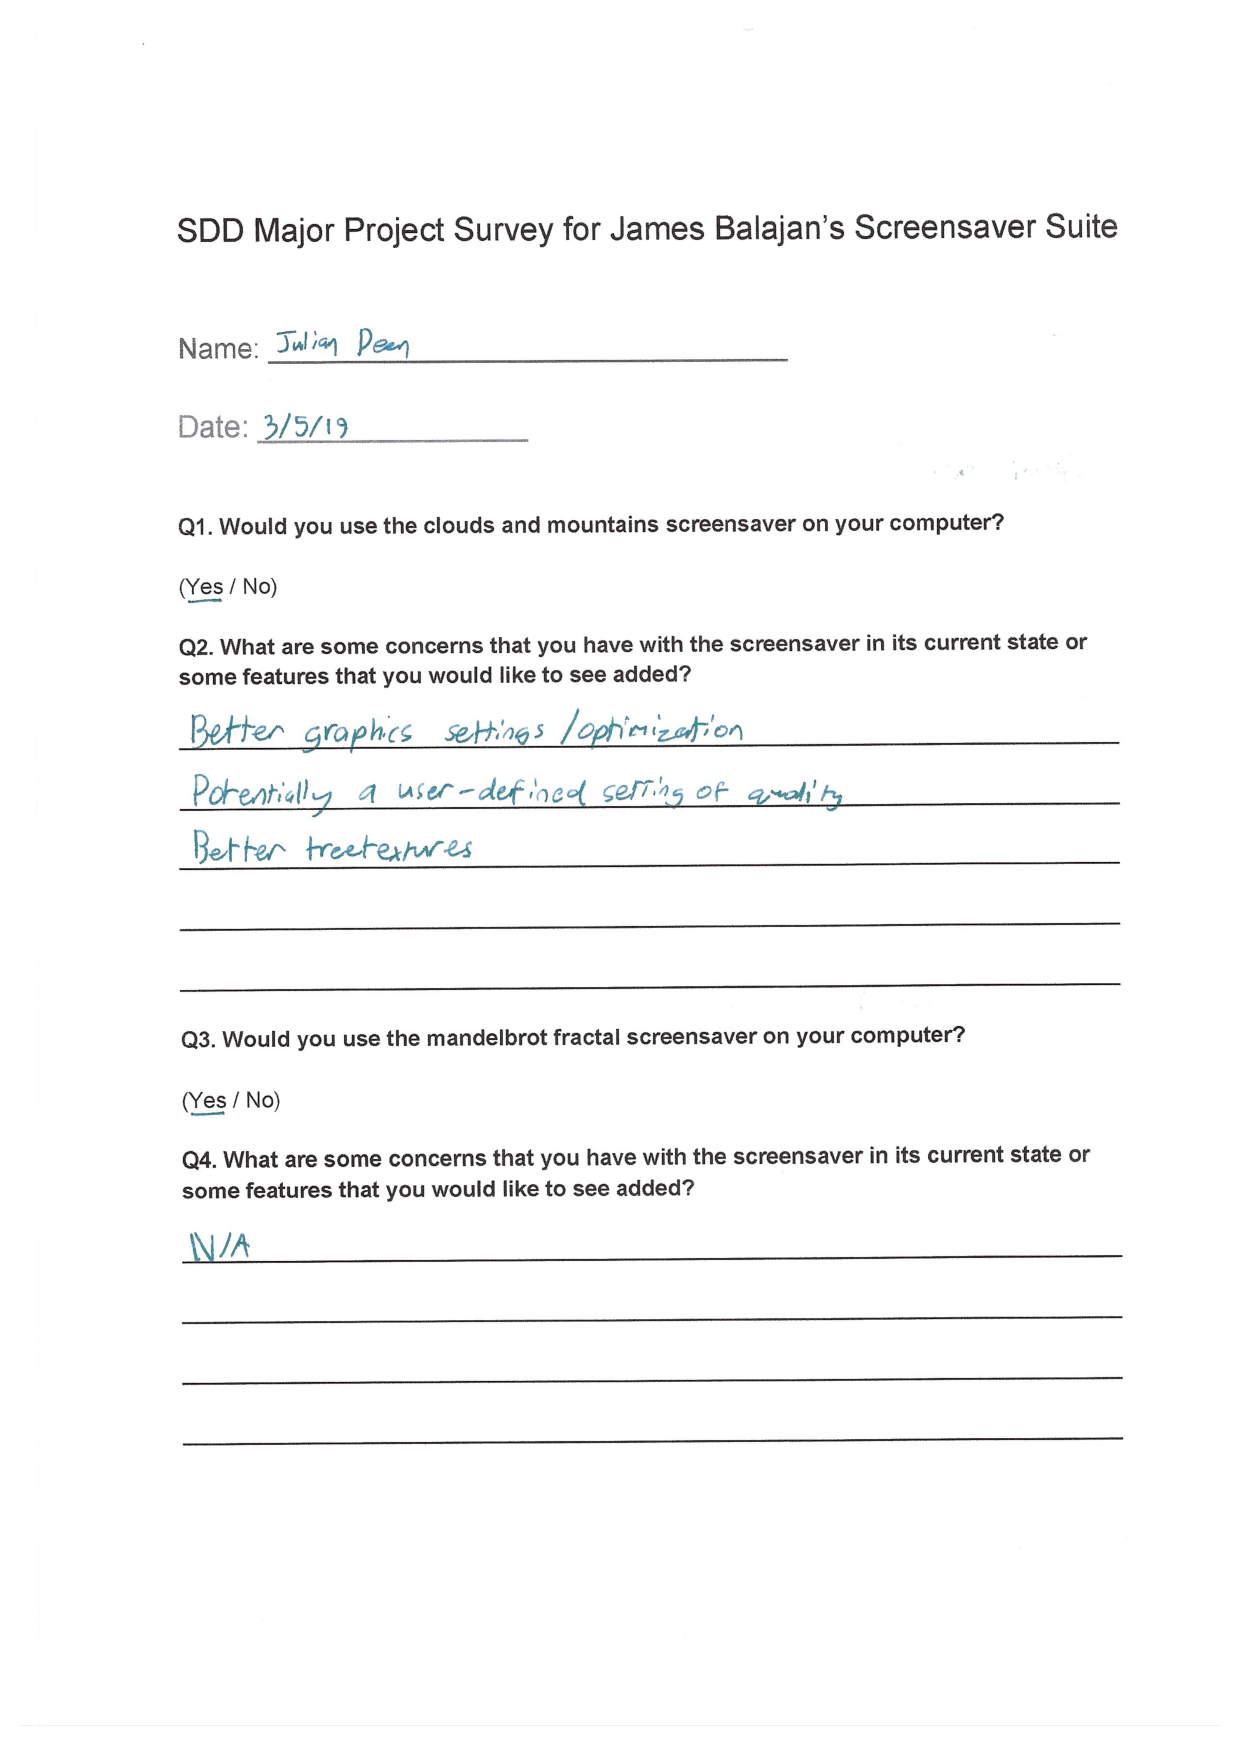
\includepdf[pages=1, scale=0.78, pagecommand={\subsection{Julian Peen - Survey Response 2} \label{app:survey-julian-2}}]{external-pdfs/JulianPeen.pdf}
\includepdf[pages=2, scale=0.78, pagecommand={}]{external-pdfs/JulianPeen.pdf}



\end{document}
